% !TEX TS-program = pdflatex
% !TEX encoding = UTF-8 Unicode

\documentclass[11pt]{report} % use larger type; default would be 10pt
\usepackage[utf8]{inputenc} % set input encoding (not needed with XeLaTeX)



%%% PAGE DIMENSIONS
\usepackage{geometry} % to change the page dimensions
\geometry{a4paper} % or letterpaper (US) or a5paper or....
% \geometry{margin=2in} % for example, change the margins to 2 inches all round
% \geometry{landscape} % set up the page for landscape
%   read geometry.pdf for detailed page layout information



\usepackage{amsmath} % AMS Math Package
\usepackage{amsthm} % Theorem Formatting
\usepackage{amssymb} % Math symbols such as \mathbb
\usepackage{graphicx} % support the \includegraphics command and options
\usepackage{color}
	%To color text, use {\color{#} text here } and the available color options include: white, black, red, 	green, blue, cyan, magenta, yellow
\usepackage{float} 
	%For Graphic Placement
		%h=here, t=top, b=bottom, p=page
		%to override latex float placement, add an ! after the line to make latex more obedient 
		%If using the float package, then using H will make latex put the graphic exactly where is it in the source code
\usepackage[colorlinks=true, linkcolor=blue, urlcolor=blue]{hyperref} 
	%To link outside a document:
		%\url{''my url''}: it will show the URL using a mono-spaced font and, if you click on it, your browser will be opened pointing at it.
		%\href{''my_url''}{''description''}: it will show the string "description" using standard document font but, if you click on it, your browser will be opened pointing at "my_url".
	%To link inside the document:
		%\hyperlink{label}{anchor caption}
		%\hypertarget{label}{link caption}

\usepackage{appendix}
\usepackage{caption}
\usepackage{subcaption}

\usepackage{minted}

\usepackage{mdwlist} %use for single spaced lists 
	%To single space lists, use the package ``mdwlist'' and then just use the commands ennumerate* and itemize* instead of the regular commands.

\setcounter{secnumdepth}{3}	% Number sub-subsections. 
\setcounter{tocdepth}{3}		% Make the Table of Contents go down to the sub-subsection level.

% \usepackage[parfill]{parskip} % Activate to begin paragraphs with an empty line rather than an indent

%%% PACKAGES
\usepackage{booktabs} % for much better looking tables
\usepackage{array} % for better arrays (eg matrices) in maths
\usepackage{paralist} % very flexible & customisable lists (eg. enumerate/itemize, etc.)
\usepackage{verbatim} % adds environment for commenting out blocks of text & for better verbatim
%\usepackage{subfig} % make it possible to include more than one captioned figure/table in a single float
% These packages are all incorporated in the memoir class to one degree or another...

%%% HEADERS & FOOTERS
\usepackage{fancyhdr} % This should be set AFTER setting up the page geometry
\pagestyle{fancy} % options: empty , plain , fancy
\renewcommand{\headrulewidth}{0pt} % customise the layout...
\lhead{}\chead{}\rhead{}
\lfoot{}\cfoot{\thepage}\rfoot{}

%%% ToC (table of contents) APPEARANCE
\usepackage[nottoc,notlof,notlot]{tocbibind} % Put the bibliography in the ToC
\usepackage[titles,subfigure]{tocloft} % Alter the style of the Table of Contents
\renewcommand{\cftsecfont}{\rmfamily\mdseries\upshape}
\renewcommand{\cftsecpagefont}{\rmfamily\mdseries\upshape} % No bold!

%%% END Article customizations



%%%%%%%%%%%%%%%%%%%%%%%%%%%%%%%%%%%%%%%%%%%%%
%LaTex Hints and Tricks
%
%
%To gather multiple equations under one number, use \begin{subequations} and \end{subequations} outside of the \begin{equation} or \begin{align}, etc. environment.
%
%To label a group of equations together, use the \begin{aligned} and \end{aligned} environments inside of the \begin{equation} and \end{equation} environment
%
% Use \numberwithin{x}{y} to number equations, etc. differently. x can be equation, figure, etc. and y can be section, subsection, etc. 
%
%Page Numbering
	%To number pages specifically, use \thispagestyle{empty} to prevent a page (usually the title) 		from being numbered
	%For frontmatter, use \setcounter{page}{1} and \pagenumbering{roman} to number pages using 		roman numerals
	%For mainmatter, use \setcounter{page}{1} and \pagenumbering{arabic} to start pages at 1
%
%
%
%Use the following to label the rows and columns of a matrix
%$$\bordermatrix{\text{corner}&c_1&c_2&\ldots &c_n\cr
%                r_1&a_{11} &  0  & \ldots & a_{1n}\cr
%                r_2& 0  &  a_{22} & \ldots & a_{2n}\cr
%                r_3& \vdots & \vdots & \ddots & \vdots\cr
%                r_4& 0  &   0       &\ldots & a_{nn}}$$
%
%To get text boxes, use \mbox (for no frame) or \fbox (for a frame)
%
%
%Font Sizes:
%    \tiny
%    \scriptsize
%    \footnotesize
%    \small
%    \normalsize
%    \large
%    \Large
%    \LARGE
%    \huge
%    \Huge 
%
%
%




%%% The "real" document content comes below...

\title{Notes on Machine Learning  \\ from Andrew Ng's Coursera Course}
\author{Simon Zahn}
\date{\today}

\begin{document}
\maketitle
\thispagestyle{empty}
\newpage

\tableofcontents
\setcounter{page}{1}
\pagenumbering{roman}


\chapter*{Preface}\addcontentsline{toc}{chapter}{Preface}

This document started out as my notes while a student in Andrew Ng's Machine Learning course on Coursera. If this subject is of any interest to you, I highly recommend you check out the course \href{https://www.coursera.org/learn/machine-learning}{here}. \\


All credit for content contained herein goes to Andrew Ng and his course. \\

In creating these notes, there are some changes I have made to the content. Primarily, I switched from using the programming language used for the course, Octave, to Python. I believe Python is a more practical choice, and it is also my programming language of choice. Additionally, by using Python, I believe I am not violating any aspect of Coursera's honor code by posting some of my solutions to the exercises. The solutions look completely different in Python, and therefore won't really be of any help to those trying to complete the course. Whether you know Python or not, the notes on the mathematics and the course content should prove useful. I also include random tidbits of ML knowledge I've picked up from other places sporadically throughout. \\

The most recent version of these notes will be kept on my GitHub page at \url{https://github.com/Sz593/coursera_ml_notes}. If you have questions or comments, you can email me at \href{mailto:simonzahn@gmail.com}{simonzahn@gmail.com}.
% \ref{chapter:metricdifferentialgeometry} (Metric Differential Geometry)

\newpage
\setcounter{page}{1}
\pagenumbering{arabic}


\chapter{Introduction}
\label{chap:introduction}

Two definitions of Machine Learning are offered at the start of the course:
\begin{description}
\item[Arthur Samuel] `The field of study that gives computers the ability to learn without being explicitely programmed.'
\item[Tom Mitchell] `A computer program is said to learn from experience $E$ with respect to some class of tasks $T$ and performance measure $P$, if its performance at tasks $T$, as measured by $P$, improves with experience $E$.'
\end{description}


\section{Supervised Learning}
\label{chapintro-sect:suplearn}

In supervised learning, we have a data set and already know what the correct output should be,  knowing that there is an existing relationship between the input and output. There are two types of supervised learning: \textbf{classification}, and \textbf{regression}. 

In a regression problem, we're trying to predict results with a continuous output; i.e. we are trying to map input variables to some continuous function. In a classification problem, we are instead trying to predict results with a discrete output. Let's look at some examples:

\begin{description}
\item[Regression] If we're trying to predict the price of a house given data about the house such as its size, location, etc., this is a regression problem. 
\item[Regression] Given a picture of a person, try to predict his/her age.
\item[Classification] Given a picture of a person, try to predict if he/she is of high school, college, or graduate age.
\item[Classification] As a bank, decide whether or not to give a loan to a potential borrower. 
\end{description}

\section{Unsupervised Learning}
\label{chapintro-sect:unsuplearn}

Unsupervised learning allows us to approach problems with little or no idea about what our results should look like. We can try and derive structure from data where we don't necessarily know the effect of the variables. We can derive this structure by clustering the data based on relationships among the variables in the data. With unsupervised learning, there is no feedback based on the prediction results.

One example of unsupervised learning is clustering. Imagine we take 1000 essays written by US college students. We can try and automatically group these essays into a smaller number that are somehow similar or related by different variables; word frequency, sentence length, page count, etc. 

Here is an example of unsupervised learning that isn't clustering: the cocktail party algorithm. This is a way to find structure in messy data, such as the identification of individual voices and music from a mesh of sounds at a cocktail party.\footnote{For more information about auditory filtering, look at Wikipedia's \href{https://en.wikipedia.org/wiki/Cocktail_party_effect}{Cocktail Party Effect} article.} 
\chapter{Linear Regression}
\label{chap:linreg}

In regression problems, we take a variable (or multiple variables) as input, and try to fit the output to a continuous expected result function. 



\section{Univariate Linear Regression}
\label{chaplinreg-sect:univar}

In univariate linear regression, we want to predict a single output value $\hat{y}$ from a single input value $x$. Since this is supervised learning, we already have an idea about what the input/output relationship should look like. 



\subsection{The Hypothesis Function}
\label{chaplinreg-sectunivar-subsect:hypfunct}

Imagine we have a problem where the input is $x$ and the output is $y$. In order to do machine learning, there should exist a relationship (a pattern) between the input and output variables. Let's say this function is $y = f\left( x \right)$. In this situation, $f$ is known as the target function. However, this function $f$ is unknown to us, so we need to try and guess what it is. To do that, we form a \textit{hypothesis} function $h\left( x \right)$ that approximates the unknown $f\left( x \right)$. 

For single variable linear regression, our hytothesis function takes two parameters: $\theta_0$ and $\theta_1$. As such, we often write it as $h_\theta\left( x \right)$, and it takes the form
\begin{equation}
\hat{y} = h_\theta\left( x \right) = \theta_0 + \theta_1 x
\end{equation}

Note that this is the equation of a straight line ($y = mx + b$). We're trying to find the values for $\theta_0$ and $\theta_1$ to get our estimated output $\hat{y}$. In other words, we're trying to determine the function $h_\theta$ that maps our input data (the $x$'s) to our output data (the $y$'s). 

Suppose we have the following set of training data:

\begin{center}
\begin{tabular}{c | c}
\textbf{Input } $x$ & \textbf{Output } $y$ \\
\hline
0 & 4 \\
1 & 7 \\
2 & 7 \\
3 & 8 \\
\end{tabular}
\end{center}

We can plot these points, as shown in Figure \ref{fig:linregeg-justpoints}. Let's make a random guess at our hypothesis function: $\theta_0  = 2$ and $\theta_1 = 2$, making our hypothesis function $h_\theta\left( x \right) = 2 + 2x$, as shown in Figure \ref{fig:linregeg-hypotguess1}.

\begin{figure}[h]
	\centering
	\begin{subfigure}[t]{0.45\textwidth}
		\centering
		\graphicspath{{./Figures/}}
		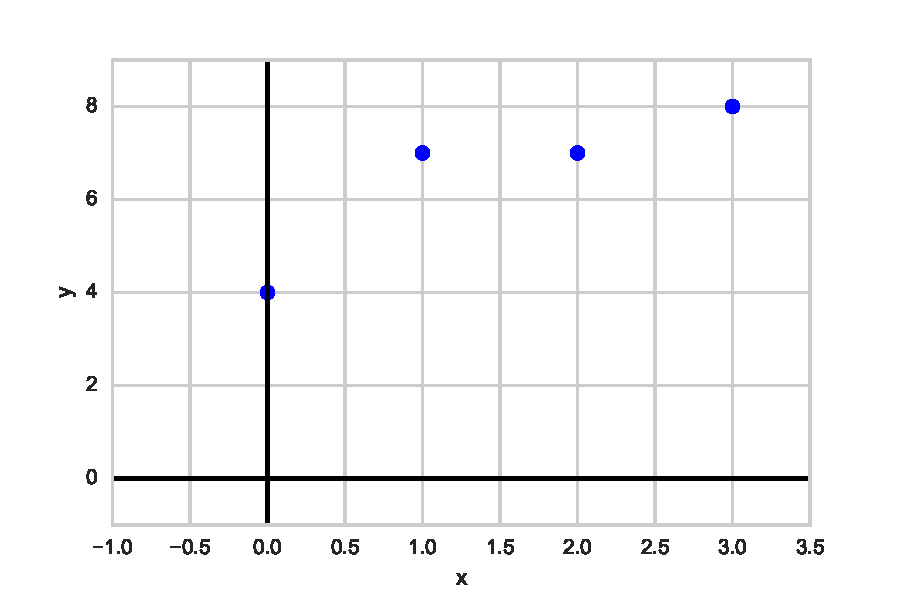
\includegraphics[scale=0.5]{linreg_eg1_plotpoints_noline.pdf}
		\caption{Plotting our example points.}
		\label{fig:linregeg-justpoints}
	\end{subfigure}
	\begin{subfigure}[t]{0.45\textwidth}
		\centering
		\graphicspath{{./Figures/}}
		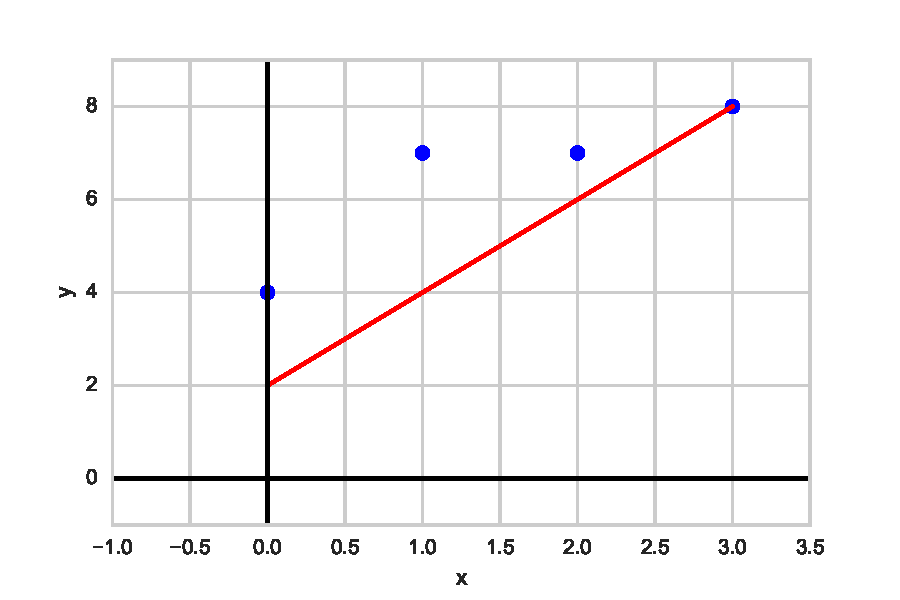
\includegraphics[scale=0.5]{linreg_eg1_plotpoints_line1.pdf}
		\caption{Plotting our example points.}
		\label{fig:linregeg-hypotguess1}
	\end{subfigure}
\end{figure}

Using this hypothesis function for $x = 1$, we have $\hat{y} = h_\theta\left( 1 \right) = 2 + 2 \cdot 1 = 4$. In this case, $\hat{y} = 4$, but $y = 7$, so mabe this isn't the best fit hypothesis.  


\subsection{The Cost Function}
\label{chaplinreg-sectunivar-subsect:costfxn}

The cost function,\footnote{The cost function can also be called the loss function.} is a function used for parameter estimation, where the input to the cost function is some function of the difference between estimated and the true values for an instance of data. In this case, we can use the cost function to measure the accuracy of our hypothesis function. 

The cost function looks at something similar to an average\footnote{It's actually something a bit fancier than a standard average.} of all the results of the hypothesis with inputs from the $x$'s compared to the actual output $y$'s. We define our cost function as follows:

\begin{equation}
J\left( \theta_0, \theta_1 \right) = \frac{1}{2m} \sum_{i=1}^m \left(\hat{y}_i - y_i \right)^2 = \frac{1}{2m} \sum_{i=1}^m \left(h_\theta\left( x_i \right) - y_i \right)^2
\end{equation}

This is known as the \textbf{mean squared error}. If we set $\bar{x}$ equal to the mean of the squares all the $ h_\theta \left( x_i \right) - y_i$, then the cost function is just the mean of $\bar{x}$. The term $\frac{1}{2m}$ is merely a convenience for the computation of gradient descent, which we'll see very shortly. 


\subsection{Gradient Descent}
\label{chaplinreg-sectunivar-subsect:graddsc}

We now have our hypothesis function defined, as well as a way of measuring how well it fits the data. Now, we have to estimate the parameters in the hypothesis function, and that's where gradient descent comes in. 

Let's graph our cost function as a function of the parameter estimates. This can be somewhat confusing, as we are moving up to a higher level of abstraction. We are not graphing $x$ and $y$ itself, but the parameter range of our hypothesis function and the cost resulting from selecting particular sets of parameters. We put $\theta_0$ on the $x$-axis, and $\theta_1$ on the $y$-axis, with the cost function on the vertical $z$-axis.

\begin{figure}[h] %  figure placement: here, top, bottom, or page
   \centering
    \graphicspath{{./Figures/}} %Use this to import an image from a subfolder.
   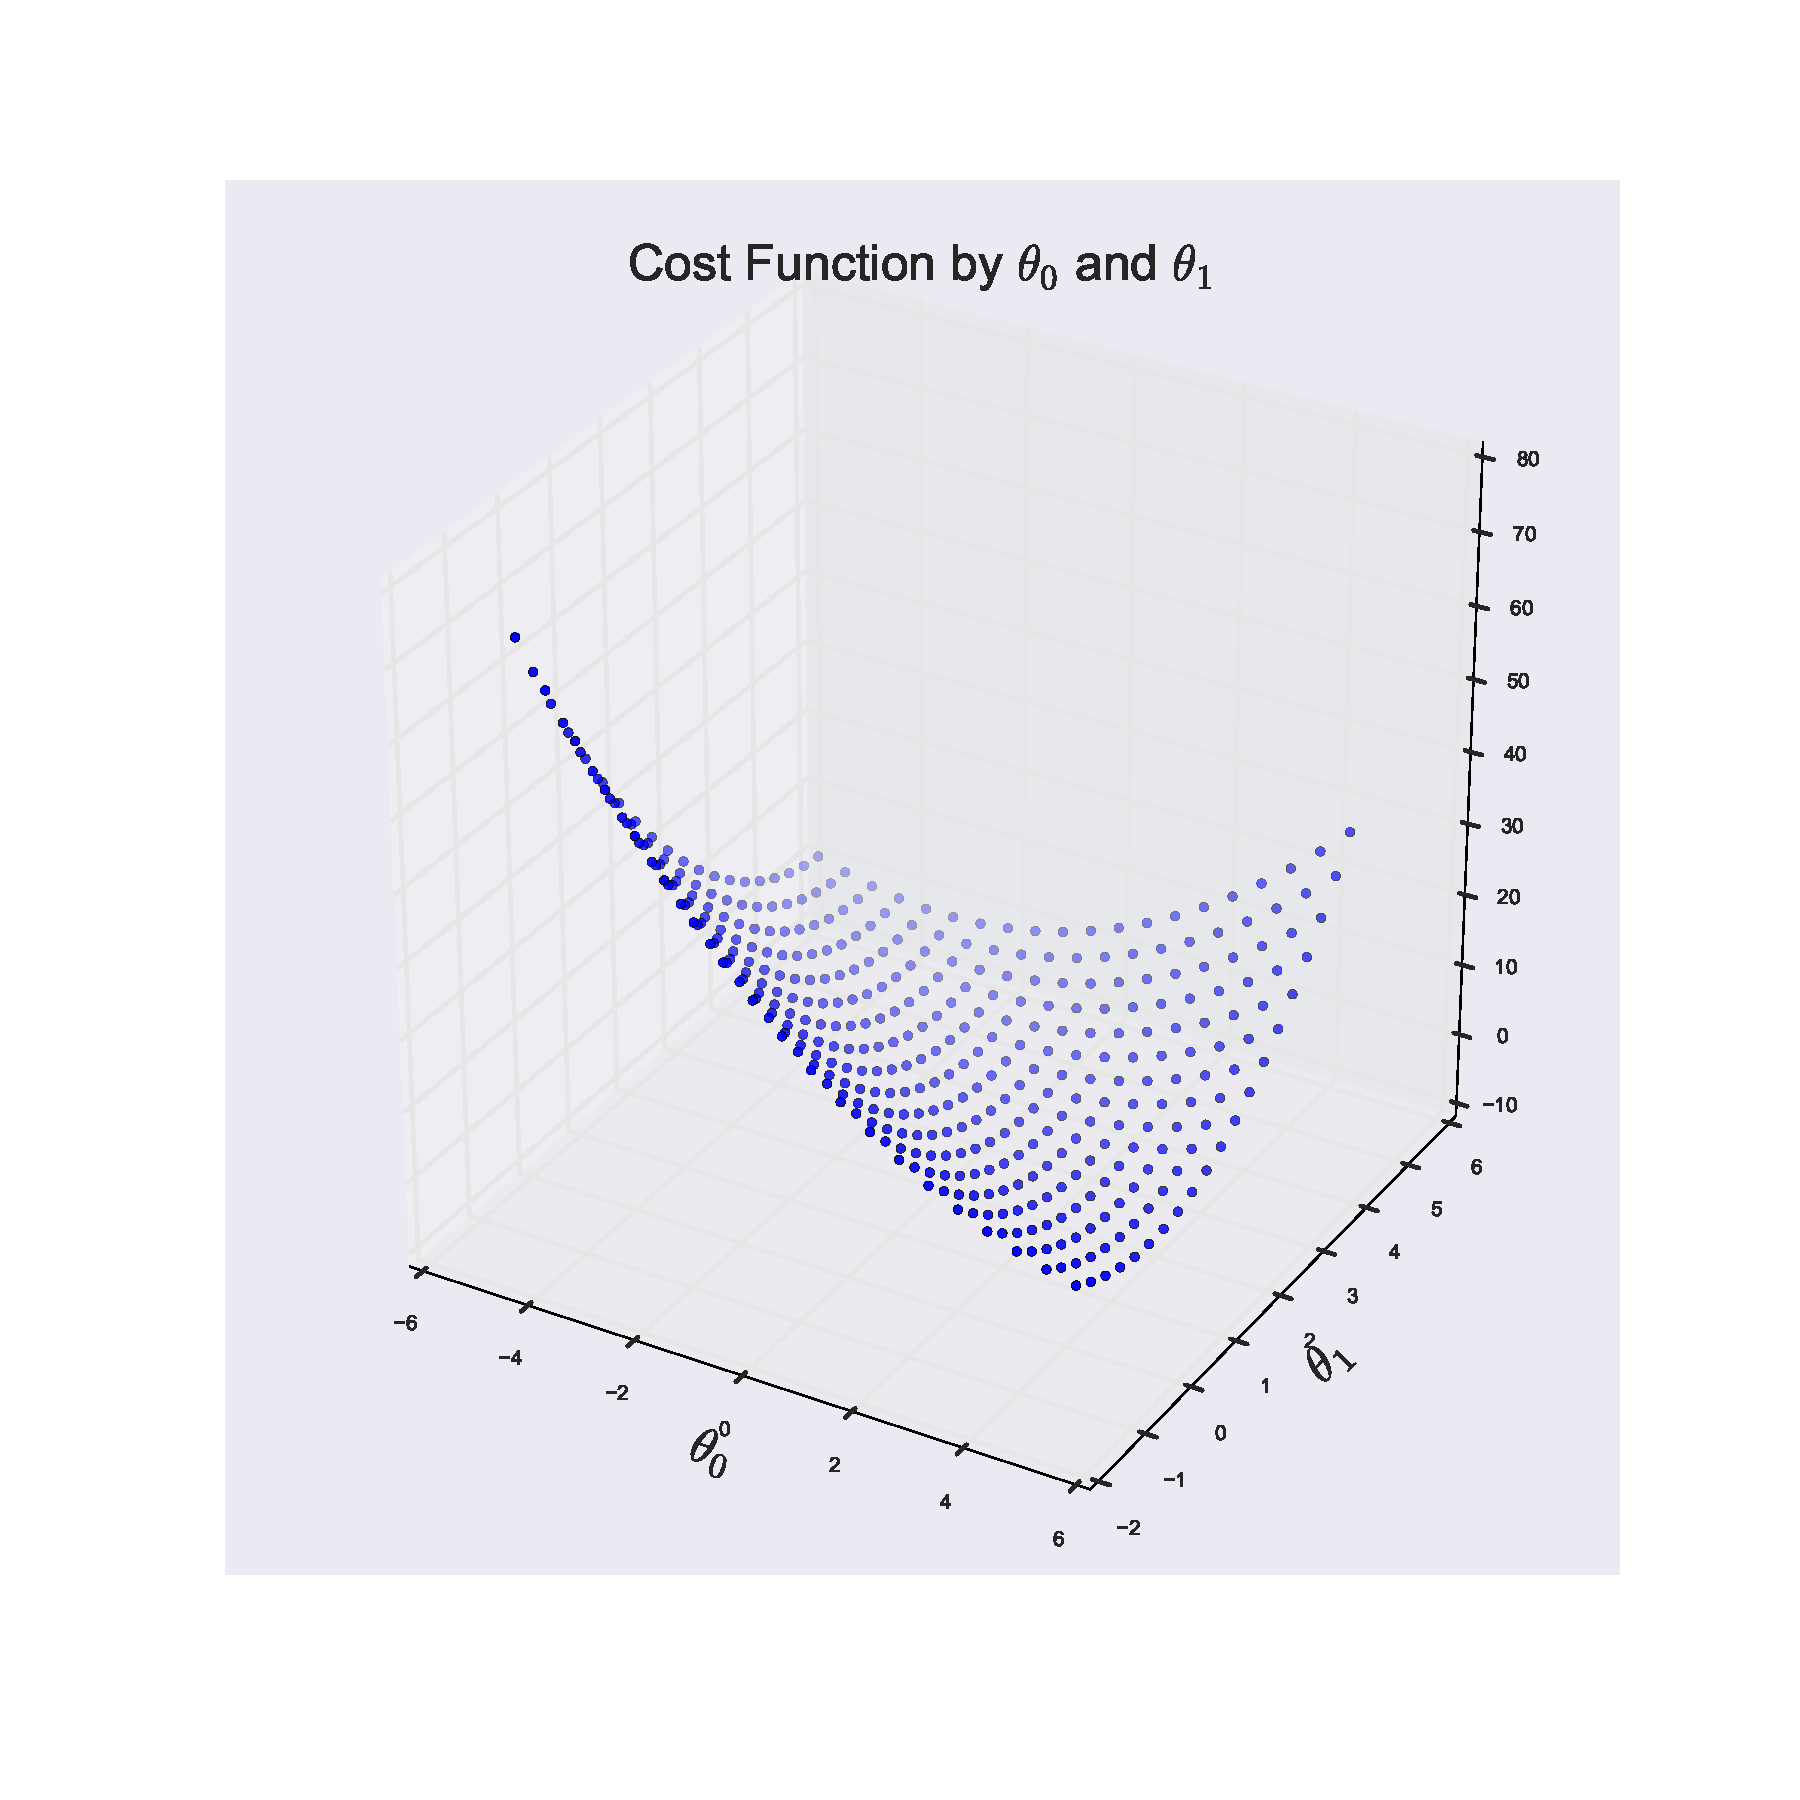
\includegraphics[scale=0.4]{linreg_eg2_cost_func_over_thetas.pdf} 
   \caption[]{Plot of the cost function $J\left(\theta_0, \theta_1 \right)$ using our hypothesis $h_\theta\left( x \right)$.}
   %If using \listoffigures command, then use \caption[short]{long}, where the short caption will appear in the list of figures, and the long caption will appear next to the figure.
   \label{s}
\end{figure}

Our goal is to take the parameters $\theta_0$ and $\theta_1$ for when the cost function is at its minimum. We can calculate this value by taking the derivative of the cost function, which gives us direction of the steepest gradient to move towards. Take a step in that direction, and repeat.The step size is determined by the parameter $\alpha$, which is called the \textbf{learning rate}. The gradient descent algorithm is:

\textbf{Repeat until convergence:}
\begin{equation}
\theta_j := \theta_j - \alpha \frac{\partial}{\partial \theta_j} J\left( \theta_0, \theta_1 \right)
\end{equation}

where $j = 0, 1$ represents the feature index number. 

\subsubsection{Gradient Descent for Linear Regression}
When specifically applied to the case of univariate linear regression, we can derive another form of the gradient descent equation. If we substitute our actual hypothesis function and cost function, we can modify the equation to

\textbf{Repeat until convergence: \{ }
\begin{equation}
\begin{aligned}
\theta_0 &:= \theta_0 - \alpha \frac{1}{m} \sum_{i=1}^m \left( h_\theta\left( x_i \right) - y_i \right) \\
\theta_1 &:= \theta_1 - \alpha \frac{1}{m} \sum_{i=1}^m \left( \left( h_\theta \left( x_i \right) - y_i \right) x_i \right)
\end{aligned}
\end{equation}

\textbf{ \} }

\noindent where $m$ is the size of the training set, $\theta_0$ is a constant that will be changing simultaneously with $\theta_1$, and $x_1$, $y_i$ are values of the given training set. Note that we have separated out the two cases for $\theta_j$ into separate equations for $\theta_0$ and $\theta_1$, and that for $\theta_1$ we are multiplying $x_i$ at the end due to the derivative. 


\section{Multivariate Linear Regression}
\label{chaplinreg-sect:multivarreg}
Let's start by looking at some sample housing data with multiple features. \\

\begin{tabular}{c | c | c | c | c }
Size (feet$^2$) & \# of Bedrooms & \# of Floors & Age (years) & Price (in 1000's of \$) \\ 
$x_1$ & $x_2$ & $x_3$ & $x_4$ & $y$ \\ \hline
2104 & 5 & 1 & 45 & 460 \\
1416 & 3 & 2 & 40 & 232 \\
1534 & 3 & 2 & 30 & 315 \\
852 & 2 & 1 & 36 & 178 \\ 
560 & 1 & 1 & 12 & 155
\end{tabular}

In this, we can introduce some notation:
\begin{itemize*}
\item The variables $x_1$, $x_2$, etc. are the features. 
\item The variable $y$ is the output variable.
\item The number of input features is denoted $n$. In this example, $n = 4$. 
\item $m$ specifies the number of training examples (rows). Here, $m = 5$.
\item $x^{\left( i \right)}$ is the input (features) of the $i^{th}$ training example. So $x^{\left( 2 \right)}$ is the column vector $[1416, 3, 2, 40, 232]$. 
\item $x_j^{\left( i \right)}$ is feature $j$ in the $i^{th}$ training example. Here, $x_1^{\left( 4 \right)} = 852$. 
\end{itemize*}

At this point, we can define the multivariable form of the hypothesis function for linear regression:
\begin{equation}
h_\theta\left( x \right) = \theta_0 + \theta_1 x_1 + \theta_2 x_2 + \theta_3 x_3 + \cdots + \theta_n x_n
\end{equation}

For convenience of notation, we will define $x_0 = 1$ for all feature vectors ($x_0^{\left( i \right)} = 1$). So now, if we include $x_0$, our hypothesis function takes the form:

\begin{equation}
h_\theta\left( x\right) = \sum_{i=0}^n \theta_i x_i
\end{equation}
Now, we can also write the $x$ values and $\theta$ values as vectors:
$$
\vec{x} = \left[ \begin{array}{c}
x_0 \\
x_1 \\
x_2 \\
\vdots \\
x_n
\end{array} \right] \in \mathbb{R}^{n+1} 
~~\mbox{\;\;\;\;\;\;\;\;\;\; and \;\;\;\;\;\;\;\;\;\;}~~
\vec{\theta} = \left[\begin{array}{c}
\theta_0 \\
\theta_1 \\
\theta_2 \\
\vdots \\
\theta_n \end{array}\right] \in \mathbb{R}^{n+1}
$$
In vector notation, this is 
\begin{equation}
h_\theta\left( x \right) = \vec{\theta}^\intercal\vec{x}
\end{equation}
where we transpose $\vec{\theta}$ into a row vector so we're able to take the inner product. 

Now that we have our vector $\vec{\theta} \in \mathbb{R}^{n+1}$, the cost function is
\begin{equation}
J\left(\vec{\theta}\right) = \frac{1}{2m}\sum_{i=1}^m \left( h_\theta\left( x^{\left( i \right)} \right) - y^{\left( i \right)} \right)^2
\end{equation}

\subsection{Gradient Descent for Multiple Variables}
Using our expanded hypothesis and cost functions, the gradient descent algorithm becomes:


\textbf{Repeat until convergence: \{ }
\begin{equation}
\theta_j := \theta_j - \alpha\frac{1}{m} \sum_{i=1}^m \left( h_\theta\left( x^{\left(i\right)} \right) - y^{\left(i\right)} \right) \cdot x_j^{\left( i \right)} ~~\mbox{\;\;\;\;\;\;\;\;\;\; for } j = 0, 1, \cdots, n
\end{equation}
\textbf{ \} }

\subsection{Feature Scaling}
When features are in very different ranges, it can slow down gradient descent dramatically (and also mess up our machine learning algorithms!), because $\theta$ will descend quickly on small ranges and slowly on large ranges, and so will oscillate inefficiently down to the minimum. The way to prevent this is to ensure that all the ranges are roughly the same, ideally:
$$ -1 \leq x \leq 1 $$

Two techniques to accomplish this are \textbf{feature scaling} and \textbf{mean normalization}. Feature scaling involved dividing the input values by the range (max value minus the min value) of the input variable, resulting in a new range of just 1. 

\begin{figure}[h] %  figure placement: here, top, bottom, or page
   \centering
    \graphicspath{{./Figures/}} %Use this to import an image from a subfolder.
   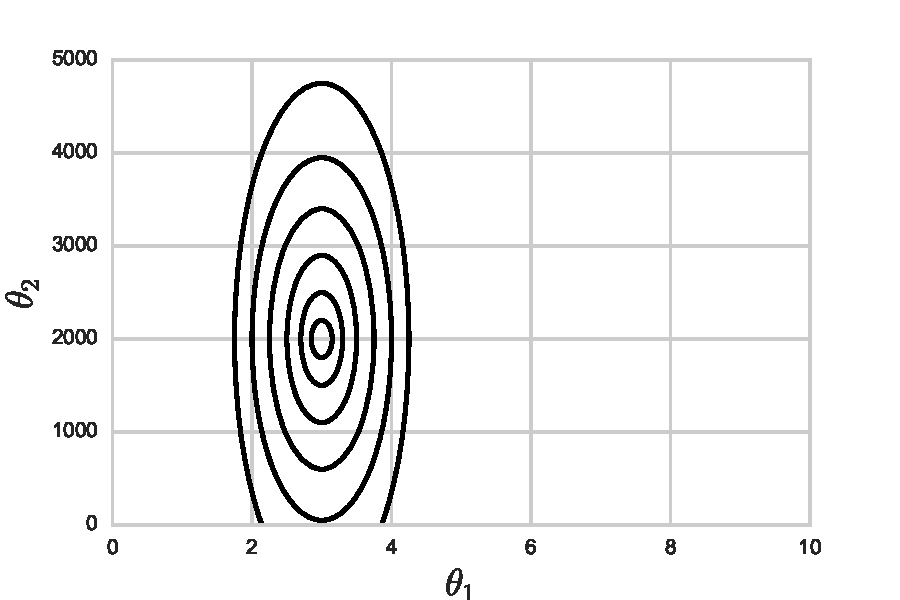
\includegraphics[scale=0.6]{linreg_eg3_why_need_feature_scaling.pdf} 
   \caption[]{When one feature is on a much larger scale than the other, the plot of the cost function will be stretched out in the direction of the larger feature. Here, imagine that $\theta_1$ is the number of bedrooms a house has, and $\theta_2$ is the size in square feet. }
   %If using \listoffigures command, then use \caption[short]{long}, where the short caption will appear in the list of figures, and the long caption will appear next to the figure.
   \label{s}
\end{figure}

Mean normalization involves subtracting the mean value for an input variable from the value for that input variable, resulting in a new mean of zero. To implement both of these simultaneously, use the following formula:
\begin{equation}
x_i := \frac{x_i - \mu_i}{s_i}
\end{equation}
where $\mu_i$ is the average value of $x_i$, and $s_i$ can either be the range ($x_\text{max} - x_\text{min}$) or the standard deviation. 


\subsection{Tips for Gradient Descent}
Here are some of Professor Andrew Ng's tips on implementing gradient descent. 

\begin{enumerate}
\item \textbf{Plot \boldmath$J\left(\theta\right)$.} If you plot $J\left(\theta\right)$ as the ordinate and the number of iterations as the abscissa,\footnote{On a Cartesian coordinate plane, the ordinate is the $y$-axis and the abscissa is the $x$-axis.} the graph should be steadily decreasing with increasing number of iterations. If $J\left(\theta\right)$ ever increases, then $\alpha$ is probably too large. 
\item If $J\left(\theta\right)$ decreases by less then $E$ in one iteration, where $E$ is some very small number, such as $10^{-3}$, then you can declare convergence. 
\item For sufficiently small $\alpha$, $J\left(\theta\right)$ should decrease with every iteration. To choose $\alpha$, try a range of values for $\alpha$ with threefold increases, such as:
$$ \cdots \to 0.001 \to 0.003 \to 0.01 \to 0.03 \to 0.1 \to 0.3 \to 1 \to 3 \to \cdots$$
\item Sometimes, it's better to define new features instead of using the ones given. For example, if we have a house with features frontage\footnote{The width of the land in the front of the house.} and depth,\footnote{The width of the land on the side of the house.} you can combine these into a new feature called area, which is how much land the house sits on.
\end{enumerate}


\subsection{Polynomial Regression}
The form of the hypothesis doesn't necessarily need to be linear of that doesn't fit the data well. We can change the behavior or curve of our hypothesis function by making it quadratic, cubic, square root, or some other form. 

For example, if our hypothesis function is $h_\theta \left(x \right) = \theta_0 + \theta_1 x_1$, we can create additional features based on $x_1$, to get the quadratic function $h_\theta\left(x\right) = \theta_0 + \theta_1 x_1 + \theta_2 x_1^2$, or the cubic function $h_\theta\left(x\right) = \theta_0 + \theta_1 x_1 + \theta_2 x_1^2 + \theta_3 x_1^3$.

When thinking about nonlinear features, it is important to keep in mind that features scaling becomes even more essential than it was for linear regression. If $x_1$ has a range of $1$ to $1000$, the $x_1^2$ has a range of $1$ to $1,000,000$.



\section{Vectorized Equations}
Let's revisit our housing example from \S \ref{chaplinreg-sect:multivarreg}. Recall that we looked at the the following example data, and we'll add an extra column for $x_0$ that always takes a value of one: \\

\begin{tabular}{c | c | c | c | c | c }
{} & Size (feet$^2$) & \# Bedrooms & \# Floors & Age (years) & Price (in \$1000's) \\ 
$x_0$ & $x_1$ & $x_2$ & $x_3$ & $x_4$ & $y$ \\ \hline
1 & 2104 & 5 & 1 & 45 & 460 \\
1 & 1416 & 3 & 2 & 40 & 232 \\
1 & 1534 & 3 & 2 & 30 & 315 \\
1 & 852 & 2 & 1 & 36 & 178 \\ 
1 & 560 & 1 & 1 & 12 & 155
\end{tabular}

From this, we construct a matrix $X$ that contains all of the features from the training data, and a vector $\vec{y}$ of all the output data. 

$$
X = \left[\begin{array}{ccccc}
1 & 2104 & 5 & 1 & 45 \\
1 & 1416 & 3 & 2 & 40 \\
1 & 1534 & 3 & 2 & 30 \\
1 & 852 & 2 & 1 & 36 \\ 
1 & 560 & 1 & 1 & 12
\end{array}\right]
~~\mbox{\;\;\;\;\;\;\;\;\;\; and \;\;\;\;\;\;\;\;\;\;}~~
\vec{y} = \left[\begin{array}{c}
460 \\ 232 \\ 315 \\ 178 \\ 155
\end{array}\right]
$$

Here, $X$ is a $m \times \left(n + 1\right)$ matrix, and $\vec{y}$ is a $m$-dimensional vector. 

Let's go through this again, but this time in full abstraction. Say we have $m$ examples $\left(x^{\left(1\right)}, y^{\left(1\right)}\right),  \left(x^{\left(2\right)}, y^{\left(2\right)}\right), \dots, \left(x^{\left(m\right)}, y^{\left(m\right)}\right)$ and each $x^{\left(i\right)}$ has $n$ features. Then, we have an $\left(n + 1\right)$-dimensional feature vector:

\begin{equation}
x^{\left(i\right)} = \left[\begin{array}{c} x_0^{\left(i\right)} \\ x_1^{\left(i\right)} \\ x_2^{\left(i\right)} \\ \vdots \\ x_n^{\left(i\right)} \end{array}\right] \in \mathbb{R}^{n+1}
\end{equation}

The matrix $X$, which is also called the \textbf{design matrix}, is constructed by taking the transpose of each vector $x^{\left(i\right)}$. Each feature vector $x^{\left(i\right)}$ becomes a row in the design matrix. Just as previously, the output vector $\vec{y}$ is obtained by taking all the labels and stacking them up into an $m$-dimensional vector, and the vector $\vec{\theta}$ is created from stacking all of the parameters for the hypothesis function. 

\begin{equation}
X = \left[\begin{array}{ccccc}
-- & -- & \left(x^{\left(1\right)}\right)^\intercal & -- & -- \\
-- & -- & \left(x^{\left(2\right)}\right)^\intercal & -- & -- \\
-- & -- & \left(x^{\left(3\right)}\right)^\intercal & -- & -- \\
-- & -- & \left(x^{\left(4\right)}\right)^\intercal & -- & -- \\
-- & -- & \vdots & -- & -- \\
-- & -- & \left(x^{\left(m\right)}\right)^\intercal & -- & -- 
\end{array}\right]
~~\mbox{\;\;\;\;\;}~~
\vec{y} = \left[\begin{array}{c} y^{\left(1\right)} \\ y^{\left(2\right)} \\ y^{\left(3\right)} \\ y^{\left(4\right)} \\ \vdots \\ y^{\left(m\right)} \end{array}\right]
~~\mbox{\;\;\;\;\;}~~
\vec{\theta} = \left[\begin{array}{c} \theta_0 \\ \theta_1 \\ \theta_2 \\ \theta_3 \\ \vdots \\ \theta_n \end{array}\right]
\end{equation}

Think back to the start of this section when we separated our table into the design matrix $X$ and the output vector $y$. The design matrix is simply the data as stored in a table put into a matrix. 

In our matrix notation for multivariate regression, the hypothesis function takes the form
\begin{equation}
h_\theta\left(X\right) = X\vec{\theta}
\end{equation}
This will always work since $X$ is an $m\times n$ matrix, and $\vec{\theta}$ is an $n \times 1$ vector. In a similar fashion, the cost function in matrix notation is
\begin{equation}
J\left(\vec{\theta}\right) = \frac{1}{2m} \left(X\vec{\theta} - \vec{y}\right)^\intercal \left(X\vec{\theta} - \vec{y}\right)
\end{equation}

The gradient descent rule can be expressed as
\begin{equation}
\vec{\theta} := \vec{\theta} - \alpha \nabla J\left(\theta\right) 
\end{equation}

There $\nabla$ is the gradient (vector derivative) operator. If we solve this out using our vectorized hypothesis function, we get
\begin{equation}
\vec{\theta} := \vec{\theta} - \frac{\alpha}{m}X^\intercal \left(X\vec{\theta} - \vec{y} \right) 
\end{equation}

\section{The Normal Equation}
The normal equation is a method of solving for the optimal $\theta$ analytically, that is, without iteration. From calculus, if we want to find the minimum of a quadratic equation, we set the derivative equal to zero, and solve. We can apply the same logic to the cost function. If we take the partial derivative $\partial/\partial \theta_j J\left(\theta\right)$ and set this equal to zero for all values of $j$, we'll analytically solve for the minimum. 

The derivation of the normal equation is fairly involved from a linear algebra perspective, so at this point just take it as a fact:
\begin{equation}
\vec{\theta} = \left( X^\intercal X \right) ^{-1} X^\intercal \vec{y}
\end{equation}

When deciding whether to use gradient descent of the normal equation, consider the following:

\begin{tabular}{| l | l |} \hline
\textbf{Gradient Descent} & \textbf{Normal Equation} \\
\hline \hline
Need to choose $\alpha$ & No need to choose $\alpha$ \\ \hline
Needs many iterations & No need to iterate \\ \hline
$O\left( kn^2 \right)$ & $O\left(n^3\right)$, need to calculate $X^\intercal X$ \\ \hline
Works well when $n$ is large & Slow if $n$ is very large \\ \hline
\end{tabular}

With the normal equation, computing the inverse has complexity $O\left( n^3 \right)$. If we have a large number of features, this will cause the normal equation to perform slowly. In practice, when $n$ exceeds $10,000$, it would probably be a good idea to use gradient descent. 

\subsection{Normal Equation Noninvertibility}
When implementing the normal equation, sometimes the matrix $X^\intercal X$ is noninvertible. The common causes are:
\begin{itemize}
\item Redundant features, where two or more features are linearly dependent
\item Too many features (i.e. $m \leq n$). In this case, delete some features or use regularization (which we'll get to later)
\end{itemize}

We typically avoid this problem by coding a pseudoinverse, instead of taking the actual inverse. 























\chapter{Logistic Regression and Regularization}

Now we turn away from regression to classification problems. Don't be confused by the name `logistic regression,' it's actually just named for the mathematical function and it's a common approach to classification.

\section{Binary Classification}
In classification problems, instead of our output being continuous, we expect it to fall into discrete classes. We'll start with the simplest case: binary classification. Here, we have our output variable $y \in \{0, 1\}$. Typically, we take $0$ as the negative class and $1$ as the positive class. 

Consider the following example: we have a sample of eight tumors, and we want to determine if they're malignant based on the tumor size. These are plotted in Figure \ref{logreg-eg-maltumor-noregline}. One thing we can do is assume a linear relationship with hypothesis $h_\theta\left( \vec{x} \right) = \vec{\theta}^\intercal \vec{x}$. This shown in Figure \ref{logreg_eg1_maltumor_linreg1}.

\begin{figure}[h]
	\centering
	\begin{subfigure}[t]{0.45\textwidth}
   		\centering
    		\graphicspath{{./Figures/}}
  		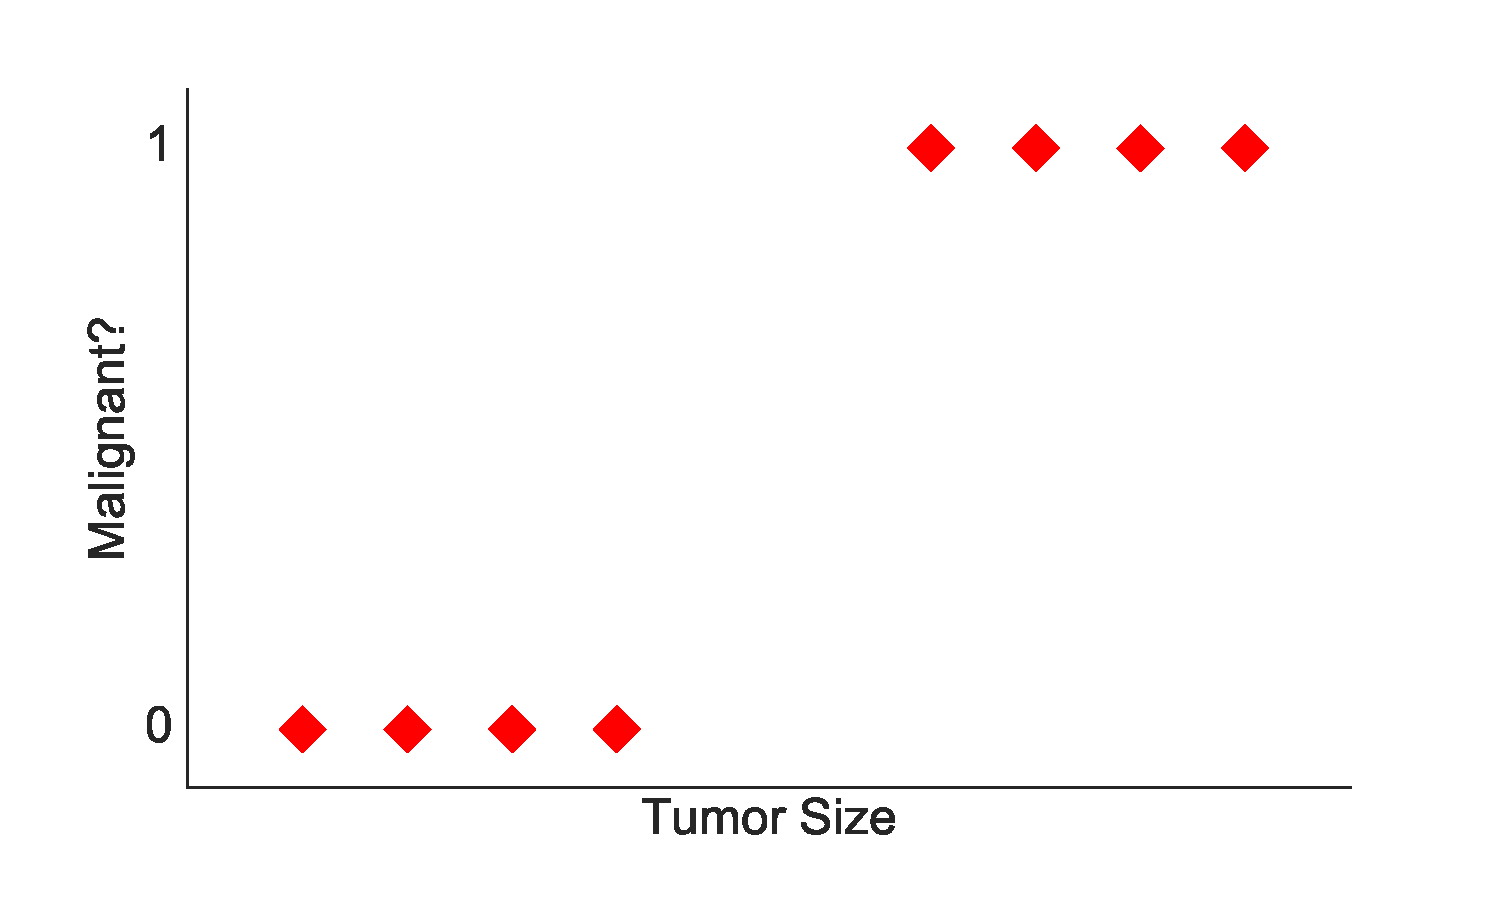
\includegraphics[scale=0.3]{logreg_eg1_maltumor.pdf} 
   		\caption[]{Sample tumor data.}
   		\label{logreg-eg-maltumor-noregline}
	\end{subfigure}
	\begin{subfigure}[t]{0.45\textwidth}
   		\centering
    		\graphicspath{{./Figures/}}
   		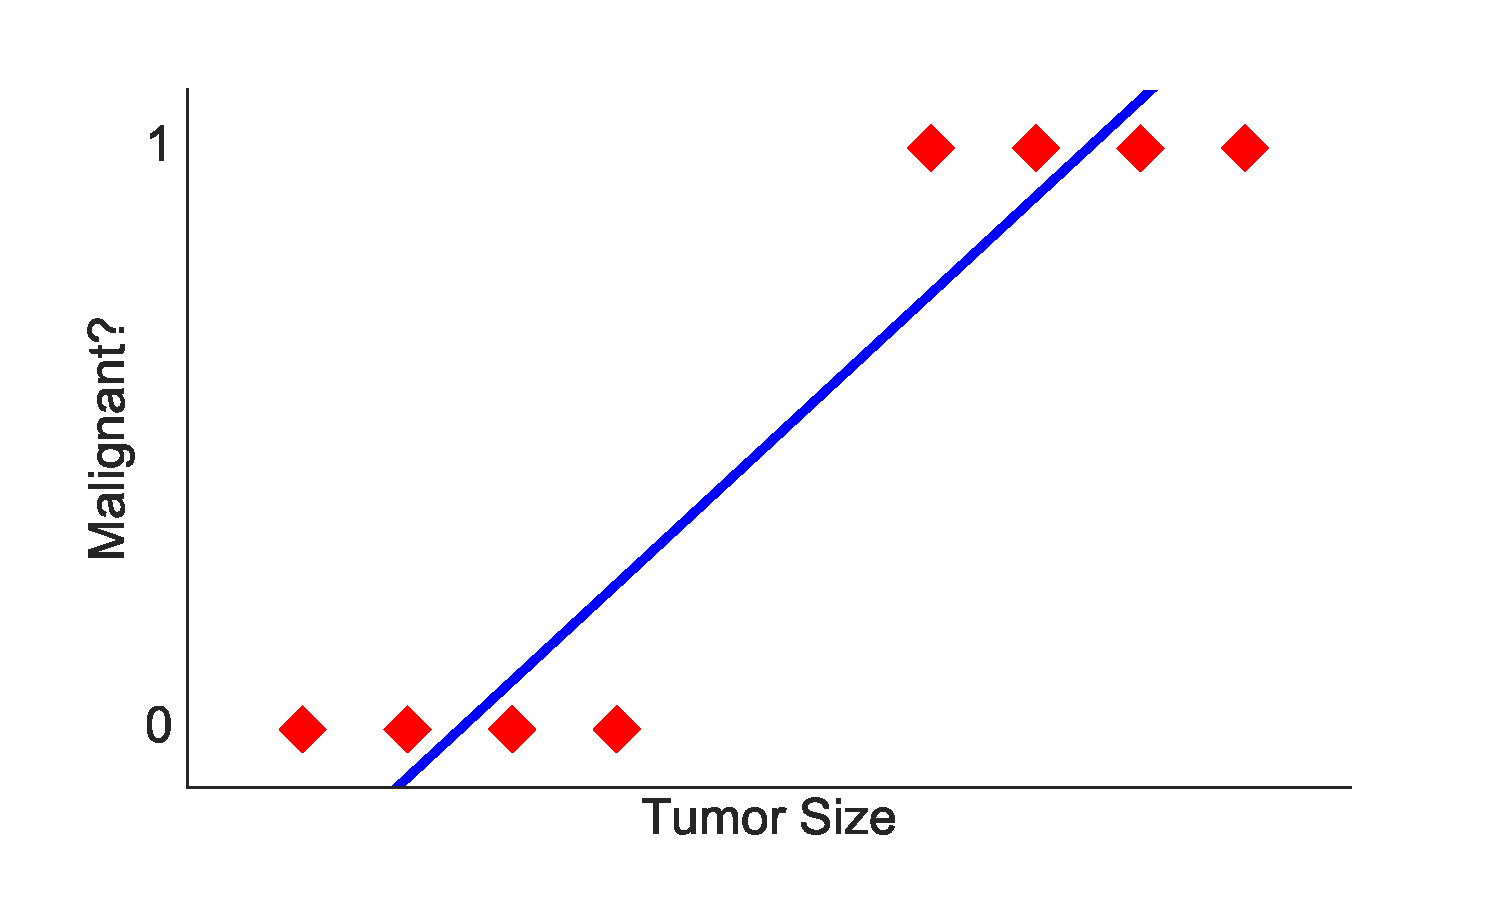
\includegraphics[scale=0.3]{logreg_eg1_maltumor_linreg1.pdf} 
   		\caption[]{Plot of tumors by size with linear regression line $y =  \frac{x-1}{6} - 0.25$.}
   		\label{logreg_eg1_maltumor_linreg1}
	\end{subfigure}
	\caption[]{Plots of tumors by size.}
\end{figure}

To try and make predictions, we can threshold the output at $h_\theta\left( x \right) = 0.5$, and then:
\begin{itemize}
\item If $h_\theta\left(x\right) \geq 0.5$, then predict $y = 1$
\item If $h_\theta\left( x \right) < 0.5$, then predict $y = 0$
\end{itemize}
and you can see this in Figure \ref{logreg_eg1_maltumor_linreg1_threshold.pdf}.

\begin{figure}[h] 
	\centering
	\graphicspath{{./Figures/}} 
	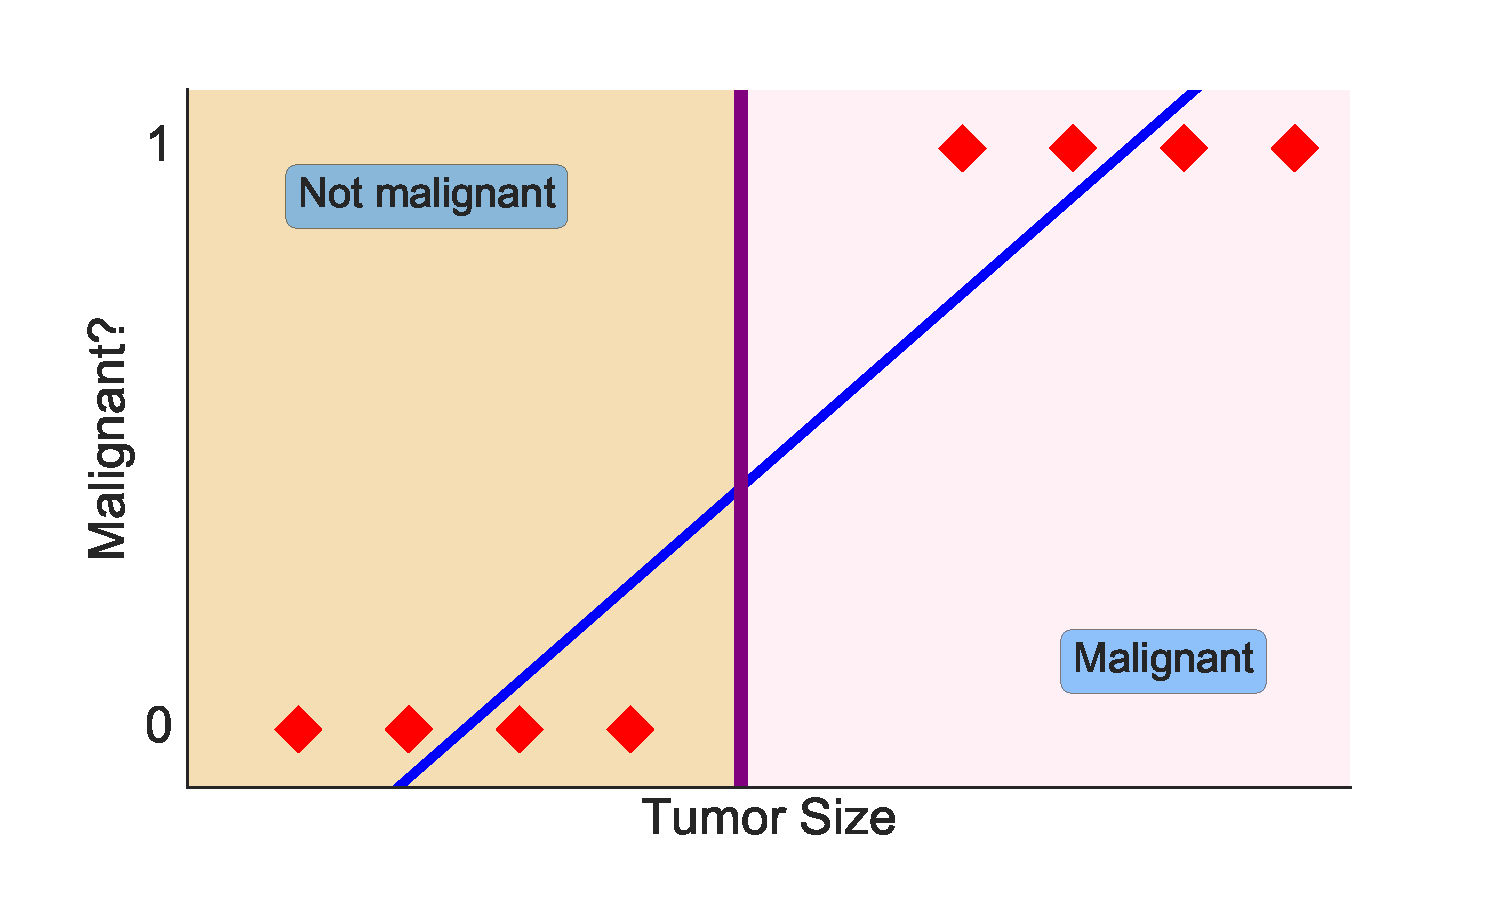
\includegraphics[scale=0.4]{logreg_eg1_maltumor_linreg1_threshold.pdf} 
	\caption[]{Linear regression plotted with classification regions. }
	\label{logreg_eg1_maltumor_linreg1_threshold.pdf}
\end{figure}


In this example, it would seem like linear regression is a good classifier. However, what if we add a new data point for a large tumor. Suddenly, our results look like this

\begin{figure}[h] %  figure placement: here, top, bottom, or page
	\centering
	\graphicspath{{./Figures/}} %Use this to import an image from a subfolder.
	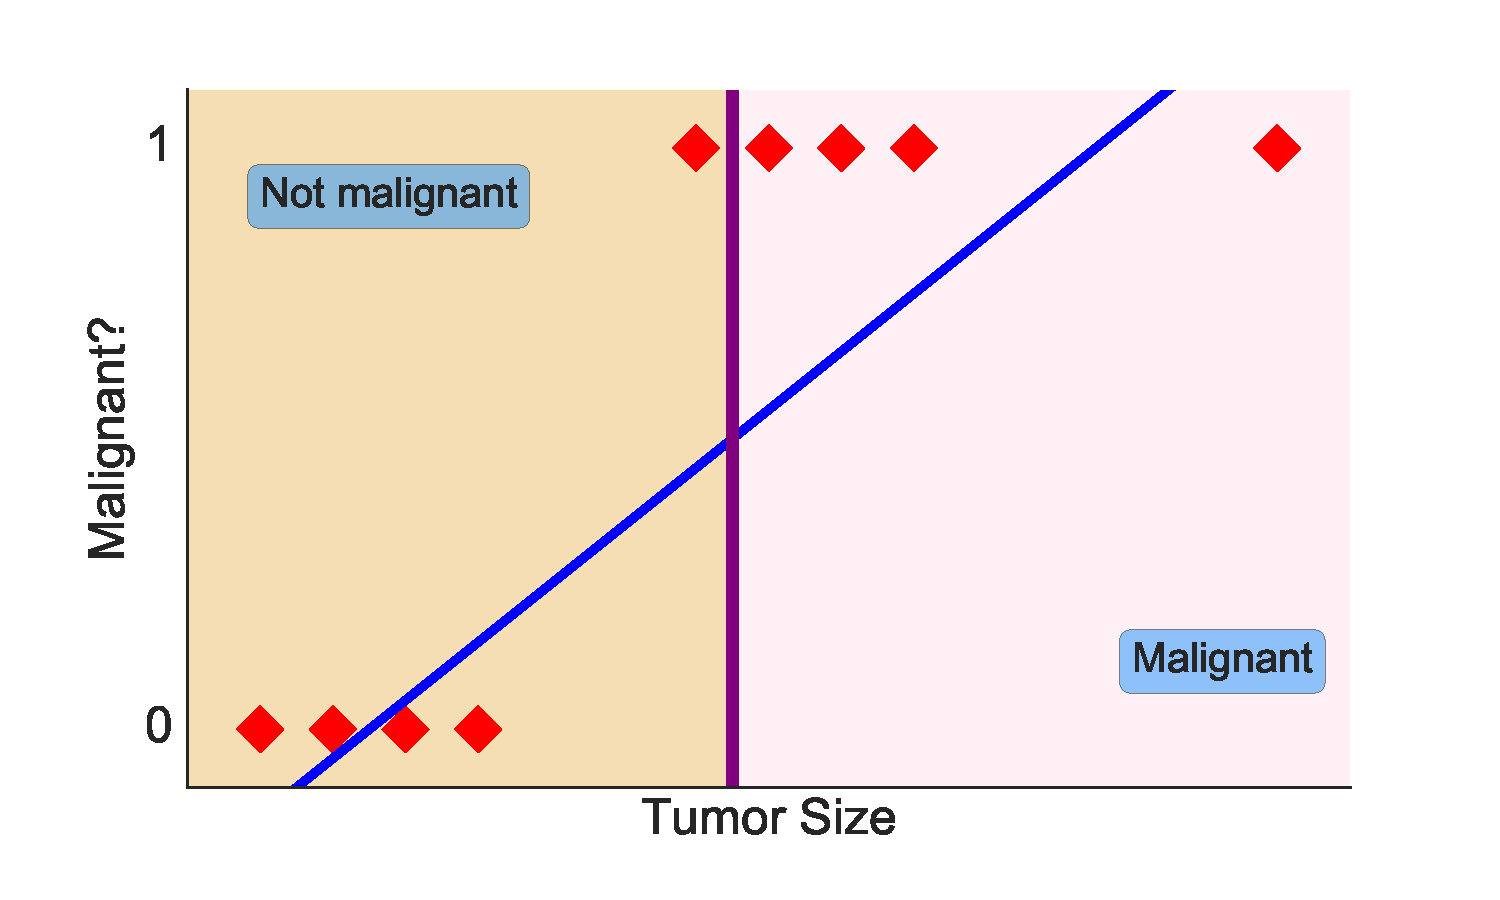
\includegraphics[scale=0.4]{logreg_eg1_maltumor_linreg1_newpoint.pdf} 
	\caption[]{Linear regression plotted with classification regions after a new data point is added. Notice how one of the malignant tumors is now being misclassified as benign.}
	\label{logreg_eg1_maltumor_linreg1_newpoint.pdf}
\end{figure}

and now, we have a malignant tumor being misclassified as benign. Ergo, maybe linear regression isn't the best way to build a binary classifier. 






\section{Hypothesis Representation}
In linear regression, our hypothesis was $h_\theta\left(\vec{x}\right) = \vec{\theta}^\intercal \vec{x}$ For logistic regression, we want our hypothesis to satisfy $0 \leq h_\theta\left(x\right) \leq 1$. To do this, we use the sigmoid function.\footnote{This is also called the logistic function, and is the namesake for logistic regression.} To make this work, we modify our hypothesis to be
\begin{equation}
h_\theta\left(x\right) = g\left(\vec{\theta}^\intercal \vec{x}\right)
\end{equation}
where the function $g\left(z\right)$ is defined as
\begin{equation}
g\left(z\right) = \frac{1}{1 + e^{-z}}
\end{equation}
Thus, to get the hypothesis function using the sigmoid function, just set $z = \vec{\theta}^\intercal \vec{x}$. 

The sigmoid function, shown in Figure \ref{logreg_eg2_sigmoid_func_plot.pdf}, maps any real number onto the interval $\left(0, 1\right)$. This makes it immensely useful for transforming an arbitrary function for use with classification.


\begin{figure}[h] %  figure placement: here, top, bottom, or page
	\centering
	\graphicspath{{./Figures/}} %Use this to import an image from a subfolder.
	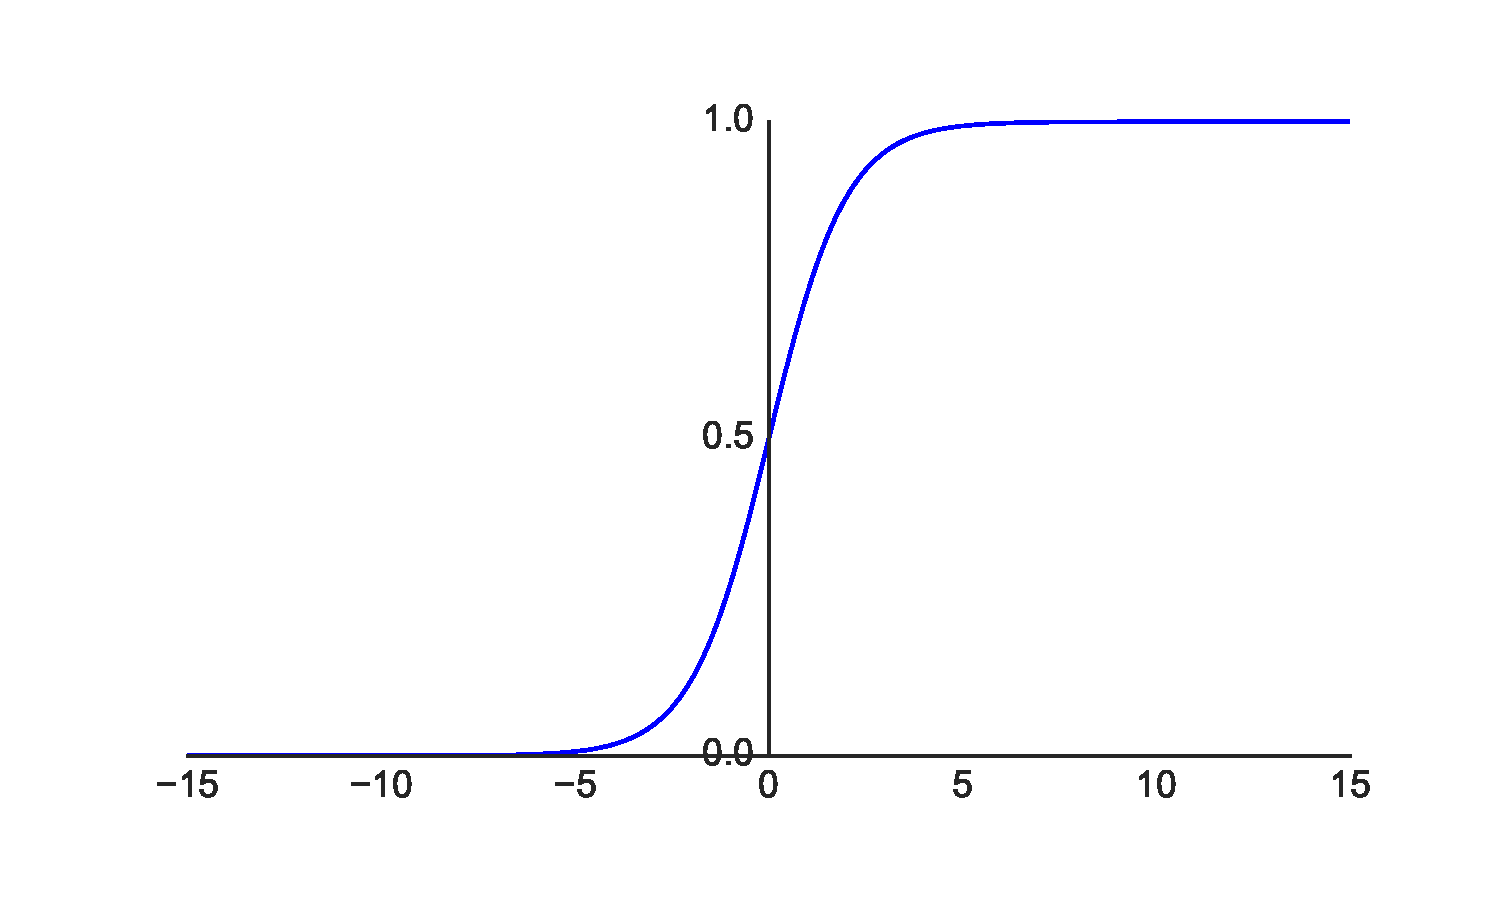
\includegraphics[scale=0.4]{logreg_eg2_sigmoid_func_plot.pdf} 
	\caption[]{Sample plot of the sigmoid function.}
	\label{logreg_eg2_sigmoid_func_plot.pdf}
\end{figure}


\subsection{Interpretation of the Logistic Hypothesis Function}

When examining the hypothesis function output for logistic regression, we interpret $h_\theta\left(x \right)$ is the estimated probability that $y=1$ on an input example $x$. For example, let's revisit the tumor size question from above. We have 
$$
\vec{x} = \left[\begin{array}{c}x_0 \\ x_1 \end{array}\right] = \left[\begin{array}{c}1 \\ \text{tumor size} \end{array}\right]
$$
If our hypothesis $h_\theta\left( x \right) = 0.7$, then we can tell the patient that there is a 70\% chance of the tumor being malignant. 

Slightly more formally, we interpret $h_\theta\left(x\right)$ as:\footnote{This is read as "the probability that $y = 1$, given $x$, parameterized by $\theta$.}
\begin{equation}
h_\theta\left(x\right) = P\left(y=1 | x; \theta\right)
\end{equation}
Thus, by the rules of probability:
\begin{align}
P\left(y=0 | x; \theta\right) + P\left(y=1 | x; \theta\right) = 1 \\
P\left(y=0 | x; \theta\right) = 1 - P\left(y=1 | x; \theta\right)
\end{align}


\subsection{Fitting Logistic Regression to a Binary Classifier}
\label{chaplogreg-sect-hyporeg-subsectbinclasfit}
Now, we need to fit our hypothesis function into a binary classfier: $0$ or $1$. Using our probabilistic interpretation of the logistic hypothesis function, we can make the following supposition:

\begin{align}
y  = 1 &\text{ given that } h_\theta\left(x\right) \geq 0.5 \\
y = 0 &\text{ given that } h_\theta\left(x\right) < 0.5
\end{align}

Recall the plot of the sigmoid function in Figure \ref{logreg_eg2_sigmoid_func_plot.pdf}. We see that $g\left(z\right) \geq 0.5$ when $z \geq 0$. In our case, if we're setting $z = \vec{\theta}^\intercal \vec{x}$, then we have:

\begin{equation}
h_\theta\left(x\right) = g\left(\vec{\theta}^\intercal\vec{x}\right) \geq 0.5 ~~\mbox{ when }~~ \vec{\theta}^\intercal\vec{x} \geq 0
\end{equation}

\noindent From this, we can now state
\begin{align}
\vec{\theta}^\intercal\vec{x} \geq 0 &\implies y = 1 \\
\vec{\theta}^\intercal\vec{x} < 0 &\implies y= 0
\end{align}

\noindent When utilizing the sigmoid function, keep the following in mind:
\begin{itemize}
\item When $z = 0$, then $e^0 = 1$ so $g\left(x\right) = \frac{1}{2}$
\item When $z$ goes to $\infty$, we have $e^{-\infty} \to 0$, and this implies $g\left(x\right) = 1$
\item As $z \to -\infty$, $e^\infty \to \infty \implies g\left(z\right) = 0$
\end{itemize}


\section{Decision Boundary}
\begin{figure}[h] %  figure placement: here, top, bottom, or page
	\centering
	\graphicspath{{./Figures/}} %Use this to import an image from a subfolder.
	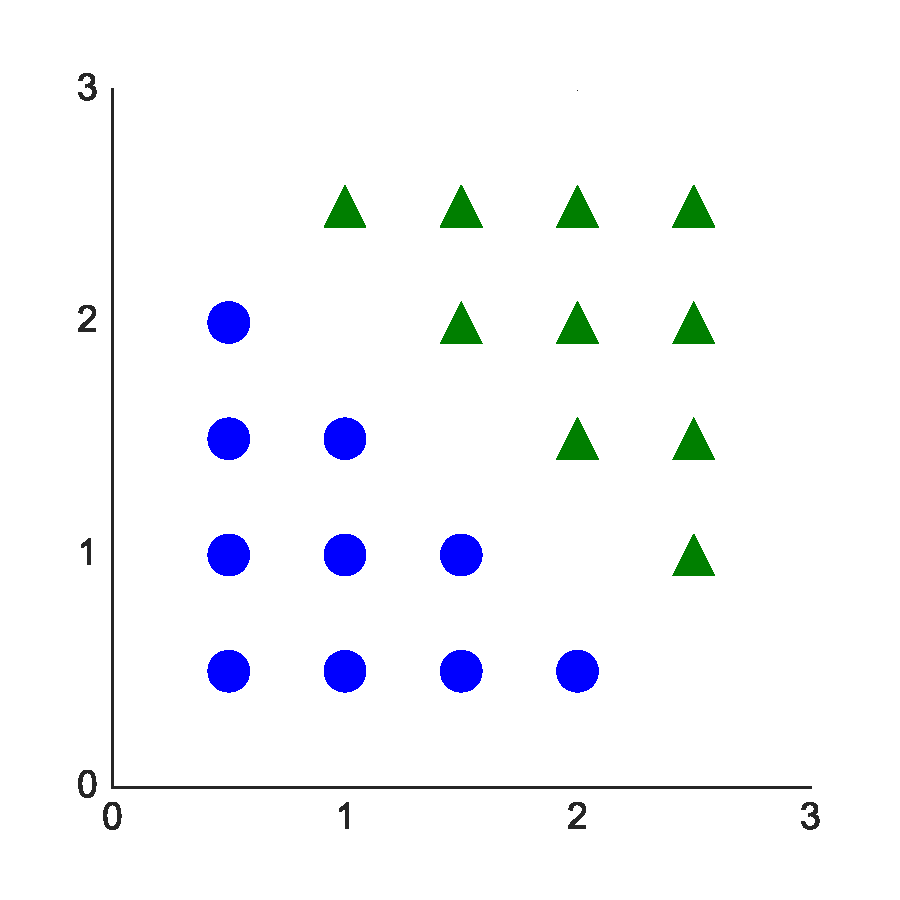
\includegraphics[scale=0.4]{logreg_eg3_decision_bndy_noline.pdf} 
	\caption[]{Sample data.}
	\label{logreg_eg3_decision_bndy_noline.pdf}
\end{figure}

Consider the data plotted in Figure \ref{logreg_eg3_decision_bndy_noline.pdf}. Suppose our hypothesis is given by
$$
h_\theta\left(x\right) = g\left(\theta_0 + \theta_1x_1 + \theta_2x_2\right)
$$
We haven't yet discussed how to fit the parameters of this model (that's coming up next), but suppose we choose the following values for the parameters
$$
\vec{\theta} = \left[\begin{array}{c}\theta_0 \\ \theta_1 \\ \theta_2\end{array}\right] = \left[\begin{array}{c} -3 \\ 1 \\ 1 \end{array}\right]
$$

Given this choice of parameters, let's figure out where $y=1$ and where $y=0$. From \S\ref{chaplogreg-sect-hyporeg-subsectbinclasfit}, recall that we predict $y=1$ when $\vec{\theta}^\intercal\vec{x} \geq 0$, so here, we predict $y=1$ if $-3 + x_1 + x_2 \geq 0$. If we solve this for $x_1 + x_2$ we get
$$
x_1 + x_2 \geq 3 \implies y = 1
$$
If we change this to a pure equality, $x_1 + x_2 = 3$, we have the equation of a straight line (shown on Figure \ref{logreg_eg3_decision_bndy_withline.pdf}). The line drawn, is called the \textbf{decision boundary}. The decision boundary is the line created by the hypothesis function that separates the area where we classify $y=0$ and where $y=1$.

\begin{figure}[h] %  figure placement: here, top, bottom, or page
	\centering
	\graphicspath{{./Figures/}} %Use this to import an image from a subfolder.
	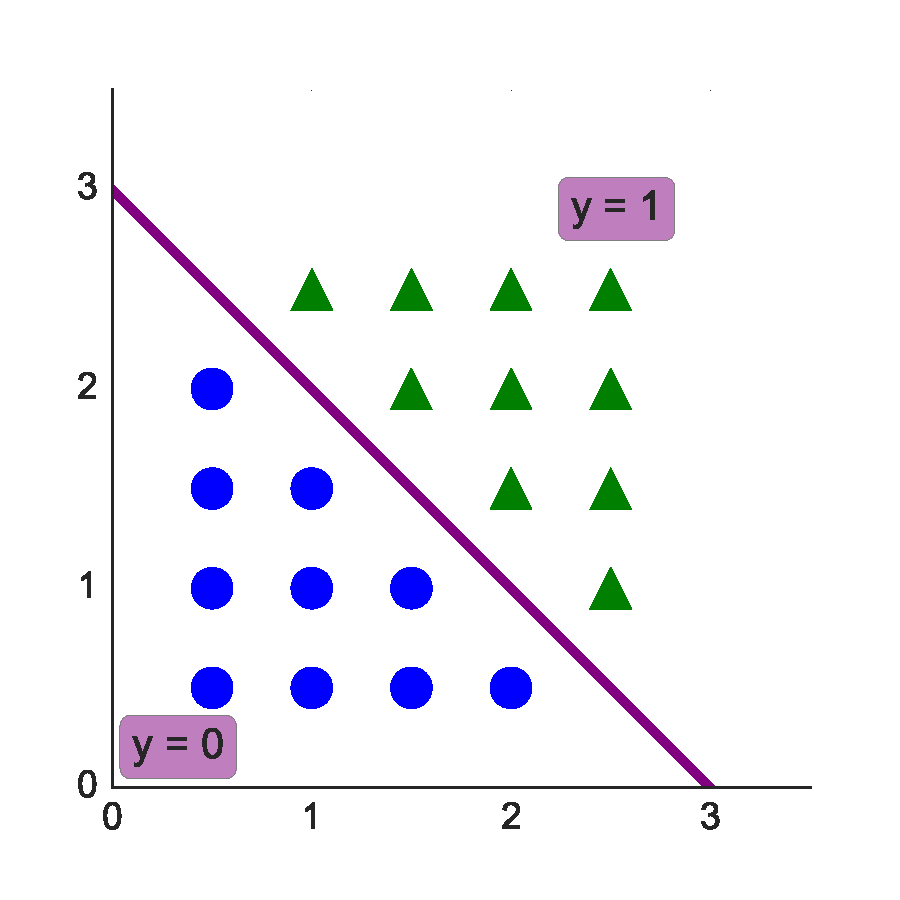
\includegraphics[scale=0.4]{logreg_eg3_decision_bndy_withline.pdf} 
	\caption[]{Some sample binary data with a plotted decision boundary. Here, the blue circles represent $y=0$, the green triangles $y=1$ and the purple line is the decision boundary.}
	\label{logreg_eg3_decision_bndy_withline.pdf}
\end{figure}

To be clean, the decision boundary is a property of the hypothesis function, and not a property of the dataset. We fit the parameters of the hypothesis based on the training data, but once those parameters are set, the decision boundary is a property solely of the hypothesis function. 

Now, suppose we have data as shown below in Figure \ref{logreg_eg3_decision_bndy_nonlinear_nocirc.pdf}. It's fairly obvious that no straight line decision boundary will work for this data. Again, we don't know how to fit the parameters for this model yet, but say our hypothesis function looks like this
$$
h_\theta\left(x\right) = g\left(\theta_0 + \theta_1x_1 + \theta_2x_2 + \theta_3x_1^2 + \theta_4x_2^2\right)
$$
Imagine we fit the parameters appropriately, and we get
$$
\vec{\theta} = \left[\begin{array}{c} \theta_0 \\ \theta_1 \\ \theta_2 \\ \theta_3 \\ \theta_4 \end{array}\right] = \left[\begin{array}{c}-1 \\ 0 \\ 0 \\ 1 \\ 1 \end{array}\right]
$$
Then, our hypothesis predicts that $y=1$ when $x_1^2 + x_2^2 \geq 1$. This is the equation for a circle of radius $1$, centered at the origin (see Figure \ref{logreg_eg3_decision_bndy_nonlinear.pdf}).
\begin{figure}[h]
	\centering
	\begin{subfigure}[t]{0.45\textwidth}
   		\centering
    		\graphicspath{{./Figures/}}
  		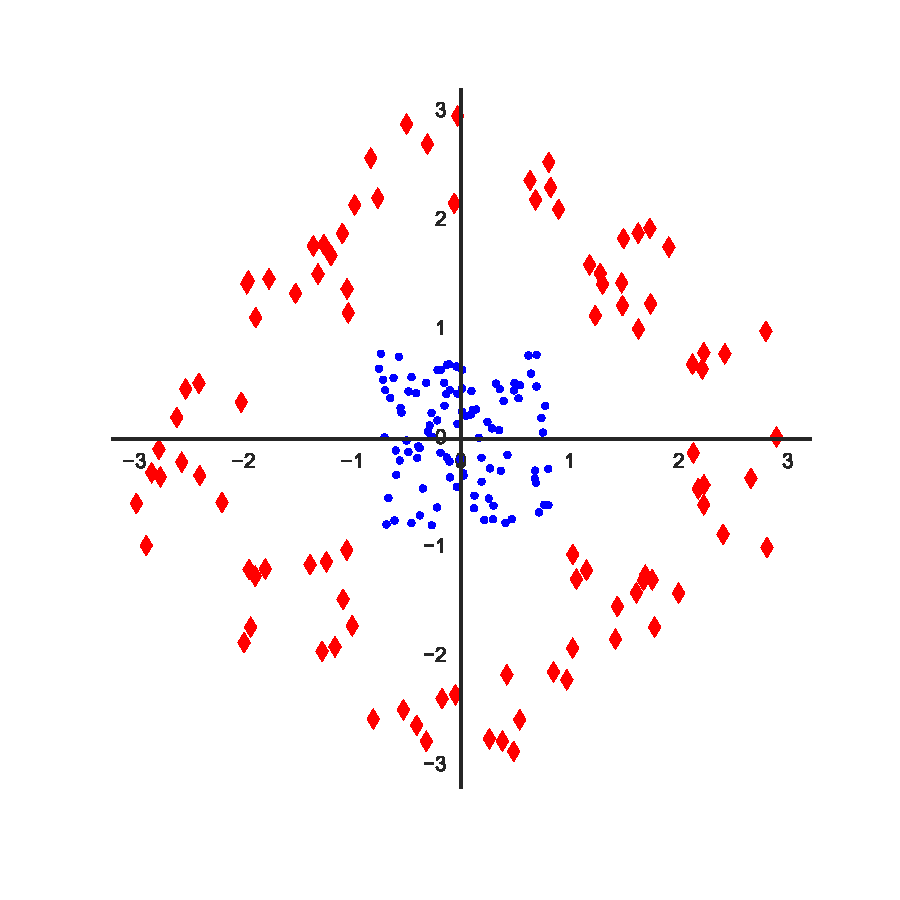
\includegraphics[scale=0.4]{logreg_eg3_decision_bndy_nonlinear_nocirc.pdf} 
   		\caption[]{This is a sample of data with no clear linear decision boundary.}
   		\label{logreg_eg3_decision_bndy_nonlinear_nocirc.pdf}
	\end{subfigure}
	\begin{subfigure}[t]{0.45\textwidth}
   		\centering
    		\graphicspath{{./Figures/}}
   		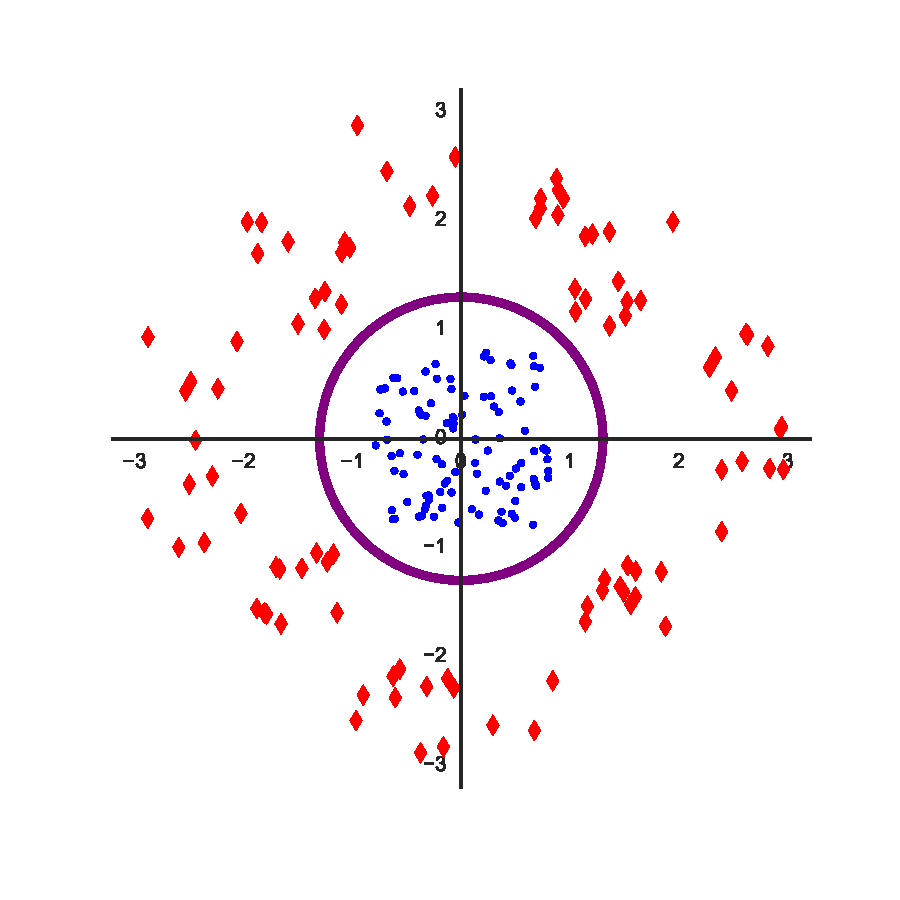
\includegraphics[scale=0.4]{logreg_eg3_decision_bndy_nonlinear.pdf} 
   		\caption[]{By altering our hypothesis function to include polynomial terms, we can have a non-linear decision boundary.}
   		\label{logreg_eg3_decision_bndy_nonlinear.pdf}
	\end{subfigure}
	\caption[]{Data that can't be fit with a linear decision line.}
\end{figure}
In this case, we predict $y=1$ everywhere outside the purple circle, and $y=0$ everywhere inside the circle. 

With even higher order polynomials, we can get even more complicated decision boundaries. 


\section{Cost Function}
Imagine we have a training set of data with $m$ examples
$$
\left\{ \left(x^{\left(1\right)}, y^{\left(1\right)}\right), \left(x^{\left(2\right)}, y^{\left(2\right)}\right), \cdots, \left(x^{\left(m\right)}, y^{\left(m\right)}\right) \right\}
$$
and $n$ features, represented by an $n+1$-dimensional feature vector
$$
x \in \left[\begin{array}{c} x_0 \\ x_1 \\ \vdots \\ x_n \end{array}\right]
$$
where $x_0 = 1$ and our output $y \in \{0, 1\}$. Our hypothesis is given by
\begin{equation}
h_\theta\left(x\right) = \frac{1}{1 + e^{-\theta^{{}^\intercal}x}}
\end{equation}
How do we choose the parameters for this model? For linear regression, we had the following cost function (adjusted slightly, we moved the $\tfrac{1}{2}$ to the inside of the summation)
\begin{equation}
J\left(\theta\right) = \frac{1}{m} \sum_{i=1}^m \frac{1}{2} \left(		h_\theta\left(x^{\left(i\right)}\right) - y^{\left(i\right)}	\right)^2
\end{equation}
but we're going to change how we write this function a little bit. Instead, we'll write
\begin{equation}
J\left(\theta\right) = \frac{1}{m} \sum_{i=1}^m \text{Cost}\left(	h_\theta\left(x^{\left(i\right)}\right), y^{\left(i\right)}\right)
\end{equation}
where we'll define the cost to be
\begin{equation}
\text{Cost}\left(	h_\theta\left(x^{\left(i\right)}\right), y^{\left(i\right)}\right) = \frac{1}{2} \left(h_\theta\left(x^{\left(i\right)}\right) - y^{\left(i\right)}	\right)^2
\end{equation}
This allows us to see more clearly that the cost function is really the sum over the cost term. To simplify even further, we'll remove the superscripts $\left(i\right)$
\begin{equation}
\text{Cost}\left(h_\theta\left(x\right), y\right) = \frac{1}{2} \left(	h_\theta\left(x\right) - y \right)^2
\end{equation}


If we try to minimize this function called Cost, it turns out to be a non-convex function. That means that the may be several local minima, which would prevent our gradient descent algorithm from working well. You can see a sample non-convex function in Figure \ref{logreg_eg4_sample_nonconvex_curve.pdf}. What we want instead, is a convex function (like a parabola) that only has a single minimum that is the global minimum. The sigmoid function is a non-linear signal function, so $J\left(\theta\right)$ ends up being non-convex. 
\begin{figure}[h] %  figure placement: here, top, bottom, or page
	\centering
	\graphicspath{{./Figures/}} %Use this to import an image from a subfolder.
	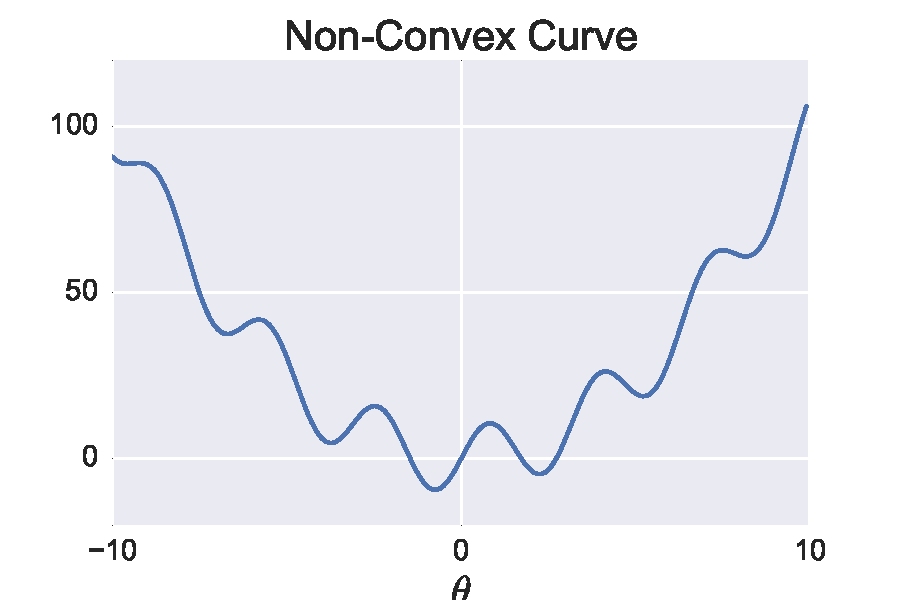
\includegraphics[scale=0.6]{logreg_eg4_sample_nonconvex_curve.pdf} 
	\caption[]{A non-convex curve. Notice all of the local minima.}
	\label{logreg_eg4_sample_nonconvex_curve.pdf}
\end{figure}

We need to define a new (convex) function that will allow us to determine the parameters in our hypothesis. For logistic regression, we use the following function
\begin{equation}
\text{Cost}\left(h_\theta\left(x\right), y\right) = \begin{cases} -\log\left(h_\theta\left(x\right)\right) & \text{if } y = 1 \\ -\log\left(1 - h_\theta\left(x\right)\right) &\text{if } y = 0 \end{cases}
\end{equation}
We plot this function below in Figure \ref{chaplogreg-sectcostfunct-plotcostfuncsample}. 

\begin{figure}[h]
	\centering
	\begin{subfigure}[t]{0.45\textwidth}
   		\centering
    		\graphicspath{{./Figures/}}
  		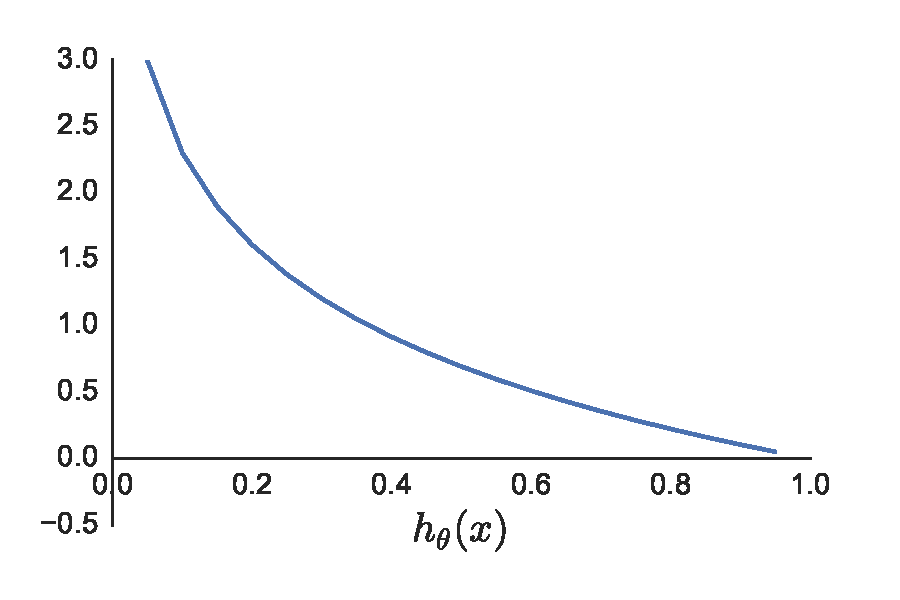
\includegraphics[scale=0.5]{logreg_eg5_cost_func_y1.pdf} 
   		\caption[]{$y=1$.}
   		\label{logreg_eg5_cost_func_y1.pdf}
	\end{subfigure}
	\begin{subfigure}[t]{0.45\textwidth}
   		\centering
    		\graphicspath{{./Figures/}}
   		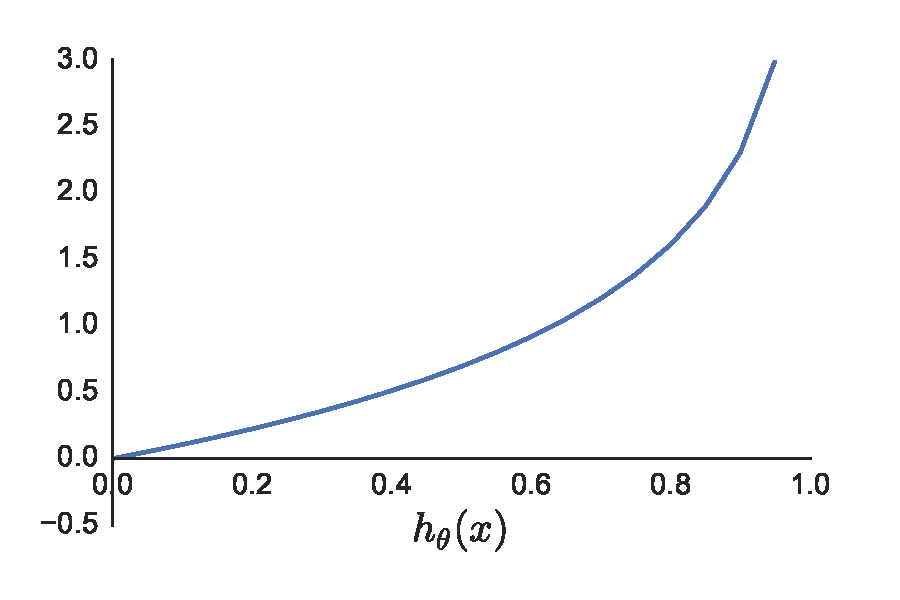
\includegraphics[scale=0.5]{logreg_eg5_cost_func_y0.pdf} 
   		\caption[]{$y=0$}
   		\label{logreg_eg5_cost_func_y0.pdf}
	\end{subfigure}
	\caption[]{The piecewise function used for the logistic regression cost function. }
	\label{chaplogreg-sectcostfunct-plotcostfuncsample}
\end{figure}

The shape of the curve comes from standard plot of $\log\left(x\right)$, and we just use a negative to flip it upside-down. This function, has some very desirable properties for us right now. 


\noindent \begin{minipage}{\linewidth}
\begin{itemize}
\item If $y = 1$, then $h_\theta\left(x\right) = 1$ and the cost is zero. However, as $h_\theta\left(x\right) \to 0$ then $\text{cost} \to \infty$. This captures the intuition that if $h_\theta\left(x\right) = 0$, but $y=1$, we'll penalize the learning algorithm by a very large cost. 
\item For $y=0$, this is reversed. If we have $y=0$ and $h_\theta\left(x\right) = 0$, then the cost is $0$. If $y=0$, the cost grows very large as $h_\theta\left(x\right)$ increases towards $1$. 
\end{itemize}
\end{minipage}


\subsection{Simplified Cost Function}
Recall our cost function 
\begin{equation}
J\left(\theta\right) = \frac{1}{m} \sum_{i=1}^m \text{Cost}\left(	h_\theta\left(x^{\left(i\right)}\right), y^{\left(i\right)}\right)
\end{equation}
where the cost is 
\begin{equation}
\text{Cost}\left(h_\theta\left(x\right), y\right) = \begin{cases} -\log\left(h_\theta\left(x\right)\right) & \text{if } y = 1 \\ -\log\left(1 - h_\theta\left(x\right)\right) &\text{if } y = 0
\end{cases}
\end{equation}
and $y \in \{0, 1\}$. 
Since $y$ is always either $0$ or $1$, we can take advantage of this to write a simplified version of our cost function:
\begin{equation}
\text{Cost}\left(h_\theta\left(x\right), y\right) = -y\log\left(h_\theta\left(x\right)\right) - \left( 1-y \right) \log\left(1 - h_\theta\left(x\right)\right)
\end{equation}
For either value of $y$, one of the terms will be multiplied by zero and disappear. So now, our cost function is\footnote{Just as an FYI, this cost function is derived statistically using maximum likelihood estimation}
\begin{align}
J\left(\theta\right) &= \frac{1}{m} \sum_{i=1}^m \text{Cost}\left(	h_\theta\left(x^{\left(i\right)}\right), y^{\left(i\right)}\right) \nonumber \\
\label{chaplogreg-sectsimpcostfunct-simpcostfuncformula}
&= -\frac{1}{m} \left[ \sum_{i=1}^m y^{\left(i\right)} \log h_\theta\left(x^{\left(i\right)}\right) + \left(1 - y^{\left(i\right)}\right) \log \left(1 - h_\theta\left(x^{\left(i\right)}\right)\right)\right]
\end{align}
We want to minimize the cost function$J\left(\theta\right)$ to fit the parameters $\theta$, so we can make our predictions using the hypothesis function. Again, we determine $\theta$ by calculating 
$$
\min_\theta J\left(\theta\right) 
$$
and predict using 
$$
h_\theta\left(x\right) = \frac{1}{1 + e^{\theta^{{}^\intercal}x}}
$$
using the calculated parameters. Now, we just need to determine how to minimize $J\left(\theta\right)$. 

\subsection{Gradient Descent for Logistic Regression}

We again return to gradient descent, of the form 


\textbf{Repeat until convergence:}
\begin{equation}
\label{chaplogreg-sectcostfunct-subsectgraddscnt-logreggraddscnt}
\theta_j := \theta_j - \alpha \frac{\partial}{\partial \theta_j} J\left( \theta \right)
\end{equation}
where we simultaneously update all $\theta_j$. If we calculate the partial derivative $\frac{\partial}{\partial \theta_j} J\left(\theta\right)$, we find
\begin{equation}
\frac{\partial}{\partial \theta_j} J\left(\theta\right) = \frac{1}{m}\sum_{i=1}^m \left( h_\theta\left(x^{\left(i\right)}\right) - y^{\left(i\right)}\right) x_j^{\left(i\right)}
\end{equation}
Plugging this back into the formula for gradient descent, we get


\textbf{Repeat until convergence:}
\begin{equation}
\theta_j := \theta_j - \frac{\alpha}{m} \sum_{i=1}^m \left( h_\theta\left(x^{\left(i\right)}\right) - y^{\left(i\right)}\right) x_j^{\left(i\right)}
\end{equation}
But wait! This looks exactly like the formula for linear regression! Is this actually a different algorithm? Yes! It is! The difference here is that the hypothesis function $h_\theta\left(x\right)$ is a different function. 

Remember that for gradient descent, we often need to apply feature scaling to make the algorithm run faster. 


\section{Vectorized Equations}
In equation \ref{chaplogreg-sectsimpcostfunct-simpcostfuncformula}, we derived a simplified version of the cost function. We can do the same thing with a vectorized implementation. First, we state the vectorized hypothesis function as
\begin{equation}
h = g\left( X\vec{\theta}\right)
\end{equation}
and then we can write the simplified cost function as
\begin{equation}
J\left(\theta\right) = \frac{1}{m}\cdot \left( -\vec{y}^\intercal \log\left(h\right) - \left(1 - \vec{y}\right)^\intercal \log \left(1 - h\right)\right)
\end{equation}
Finally, we write out the vectorized form for gradient descent
\begin{equation}
\vec{\theta} := \vec{\theta} - \frac{\alpha}{m}X^\intercal \left( g\left(X\vec{\theta}\right) - \vec{y}\right)
\end{equation}

\section{Advanced Optimization}

There are other, more sophisticated algorithms that are able to more quickly optimize $\theta$. These algorithms are a little more complicated, so you shouldn't try to write them yourself unless you're an expert in numerical computing. 

In particular, there are three algorithms that we'll mention:
\begin{itemize}
\item Conjugate gradient algorithm
\item Broyden-Fletcher-Goldfarb-Shanno (BFGS) algorithm
\item L-BFGS-B
\end{itemize}
In Python, these algorithms (and several others) are available in the {\tt scipy.optimize} package. The algorithm is chosen using the {\tt method='X'} flag, where X can be CG, BFGS, or L-BFGS-B, respectively, to use any of the above algorithms. 
\begin{minted}{python}
from scipy.optimize import minimize
\end{minted}
We'll go through an example or two in the coding section.

%%%%%%%%%%%%%%%%%%%%%%%%
%								%
%		Add hyperlink to coding			%
%								%
%%%%%%%%%%%%%%%%%%%%%%%%


\section{Multiclass Classification: One-vs-All}

What is a multiclass classification problem? Here are some examples:
\begin{itemize}
\item You want to build an algorithm to automatically tag your email with different categories: work, friends, family, and hobby. Here, you have a classification problem for four classes. 
\item For a medical visit, you might want to classify patients into not ill, having a cold, or having the flu. 
\item To build an algorithm that classifies the weather into sunny, cloudy, rain, and snow.
\end{itemize}
\begin{figure}[h]
	\centering
	\begin{subfigure}[t]{0.45\textwidth}
   		\centering
    		\graphicspath{{./Figures/}}
  		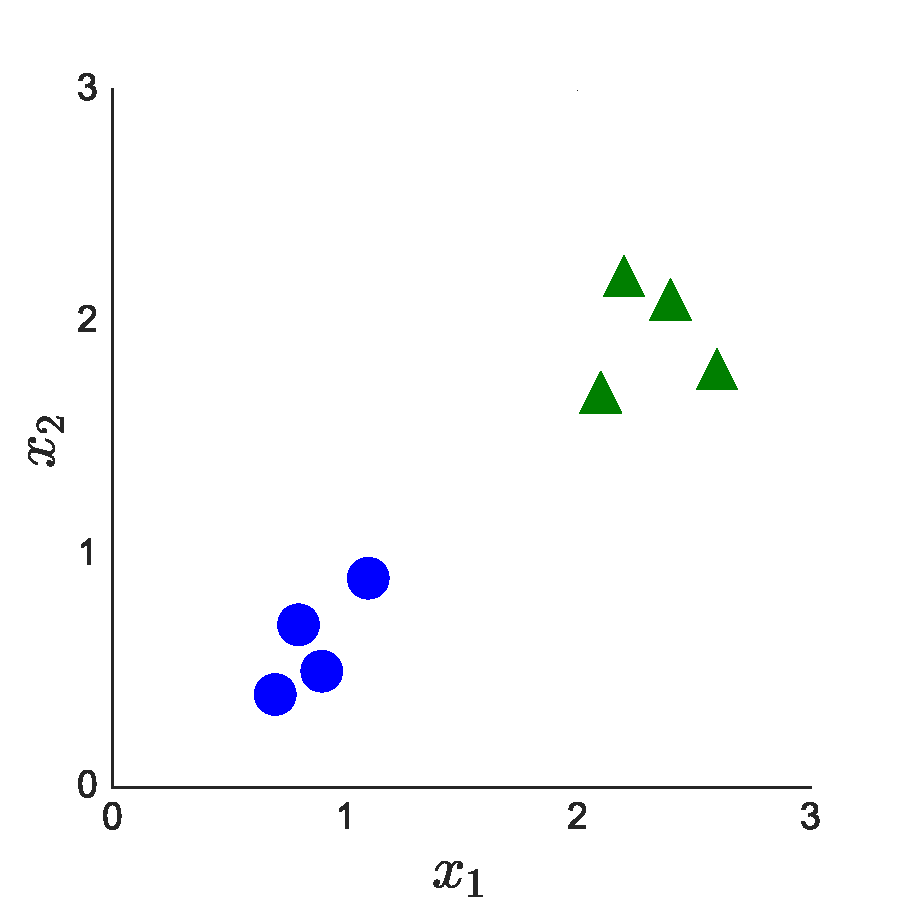
\includegraphics[scale=0.45]{logreg_eg6_binary_eg_data.pdf} 
   		\caption[]{Binary Classification}
   		\label{logreg_eg6_binary_eg_data.pdf}
	\end{subfigure}
	\begin{subfigure}[t]{0.45\textwidth}
   		\centering
    		\graphicspath{{./Figures/}}
   		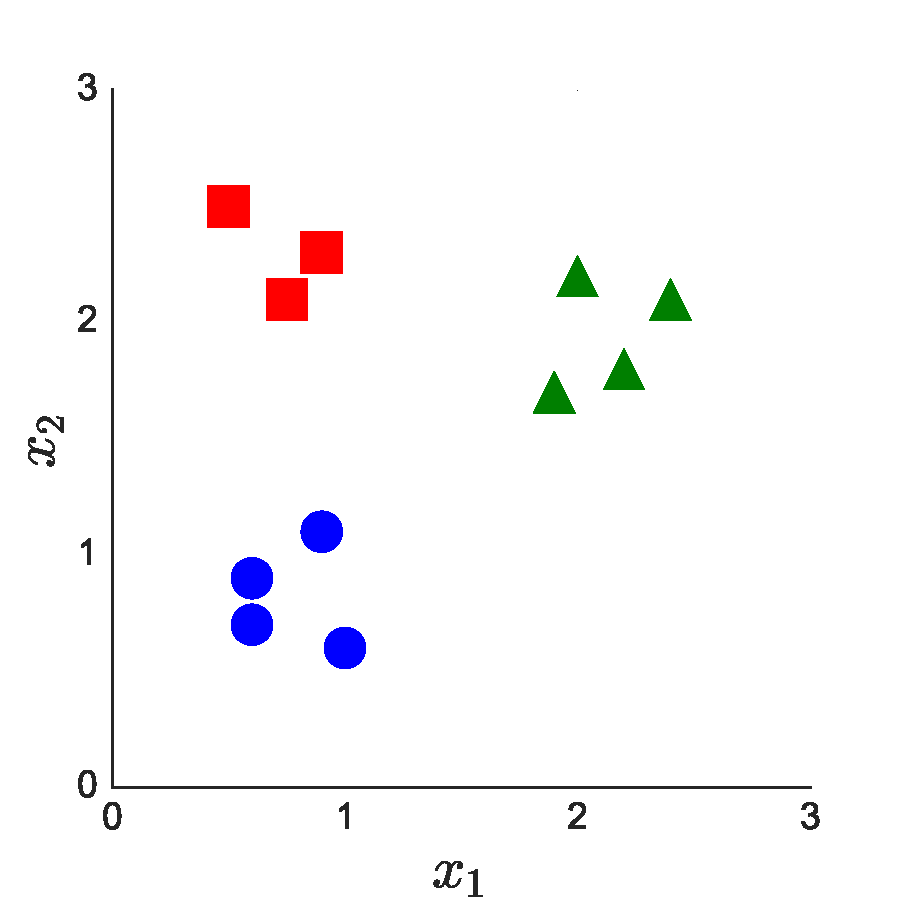
\includegraphics[scale=0.45]{logreg_eg6_multiclass_eg_data.pdf} 
   		\caption[]{Multiclass Classification}
   		\label{logreg_eg6_multiclass_eg_data.pdf}
	\end{subfigure}
	\caption[]{Examples of binary and multiclass classification.}
%	\label{}
\end{figure}
Previously, for a binary classification problem, our data looked like the data in Figure \ref{logreg_eg6_binary_eg_data.pdf}, with multiclass classification, the data looks more like Figure \ref{logreg_eg6_multiclass_eg_data.pdf}.
\begin{figure}[h] %  figure placement: here, top, bottom, or page
	\centering
	\graphicspath{{./Figures/}} %Use this to import an image from a subfolder.
	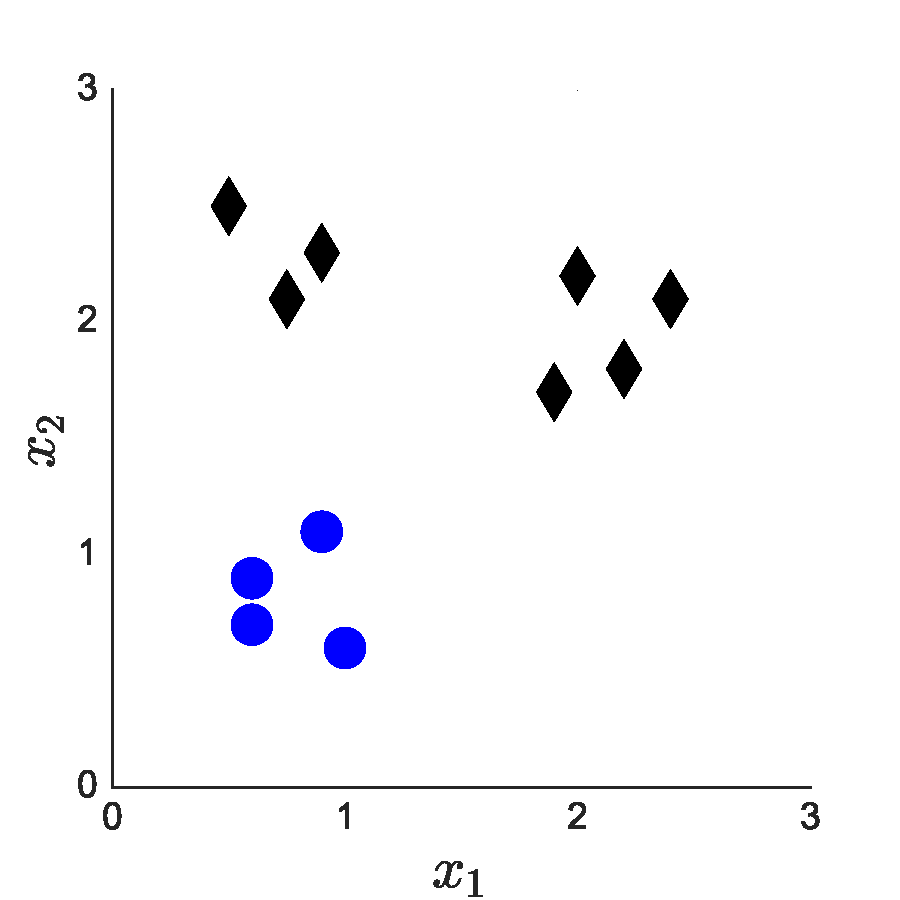
\includegraphics[scale=0.45]{logreg_eg6_multiclass_onevall_step1.pdf} 
	\caption[]{One-vs-all classification. We're selecting one class to be our positive class, and the rest all become the negative class.}
	\label{logreg_eg6_multiclass_onevall_step1.pdf}
\end{figure}

We know how to perform binary classification, but how to we make this work with more classes? We can use the idea of one-vs-all classification.\footnote{This can also be called one-vs-rest classification.} Here's how it works; let's say we have a training set of three classes (such as in Figure \ref{logreg_eg6_multiclass_eg_data.pdf}). What we can do is turn this into three separate binary classification problems.\footnote{If we have $n$ different classes, our problem splits into $n+1$ different binary classification problems.This is because the vector $\vec{y}$ starts at index $0$, so $\left|\left|\vec{y}\right|\right| = n+1$.} Start by picking a class, say the blue circles, and make it our positive class; then lump all the other data into the negative class (see Figure \ref{logreg_eg6_multiclass_onevall_step1.pdf}).

We fit a classifier to this, called $h_\theta^{\left(1\right)}\left(x\right)$. We then do this for the two other classes, and fit them to logistic regression classifiers $h_\theta^{\left(2\right)}\left(x\right)$ and $h_\theta^{\left(3\right)}\left(x\right)$. Here, we've fit three classifiers
\begin{equation}
h_\theta^{\left(i\right)}\left(x\right) = P\left(y=i | x; 0\right)	~~\mbox{\;\;\;\;\;\;\;\;\;\; for } i = \{1, 2, 3\}
\end{equation}
that are trying to estimate the probability that $y$ is equal to class $i$, given $x$ and parameterized by $\theta$. So  $h_\theta^{\left(i\right)}\left(x\right)$ is trying to estimate the probability that a data point is of class $i$. 

For a new input $x$, to make a prediction, we pick the class $i$ that maximizes 
\begin{equation}
\max_i  h_\theta^{\left(i\right)}\left(x\right)
\end{equation}
and this tells us which class to assign the new input to. 





\section{Regularization}
For the two machine learning algorithms we've seen so far, they tend to work pretty well. But when applied to specific datasets, they can run into a problem called overfitting, and this can cause them to perform very poorly. We're going to discuss a little more detail about this problem, and then go into ways to ameliorate it and increase our algorithm performance. Let's plot some housing data, and then take a look at three potential regressions. 

\begin{figure}[h]
	\centering
	\begin{subfigure}[t]{0.3\textwidth}
   		\centering
    		\graphicspath{{./Figures/}}
  		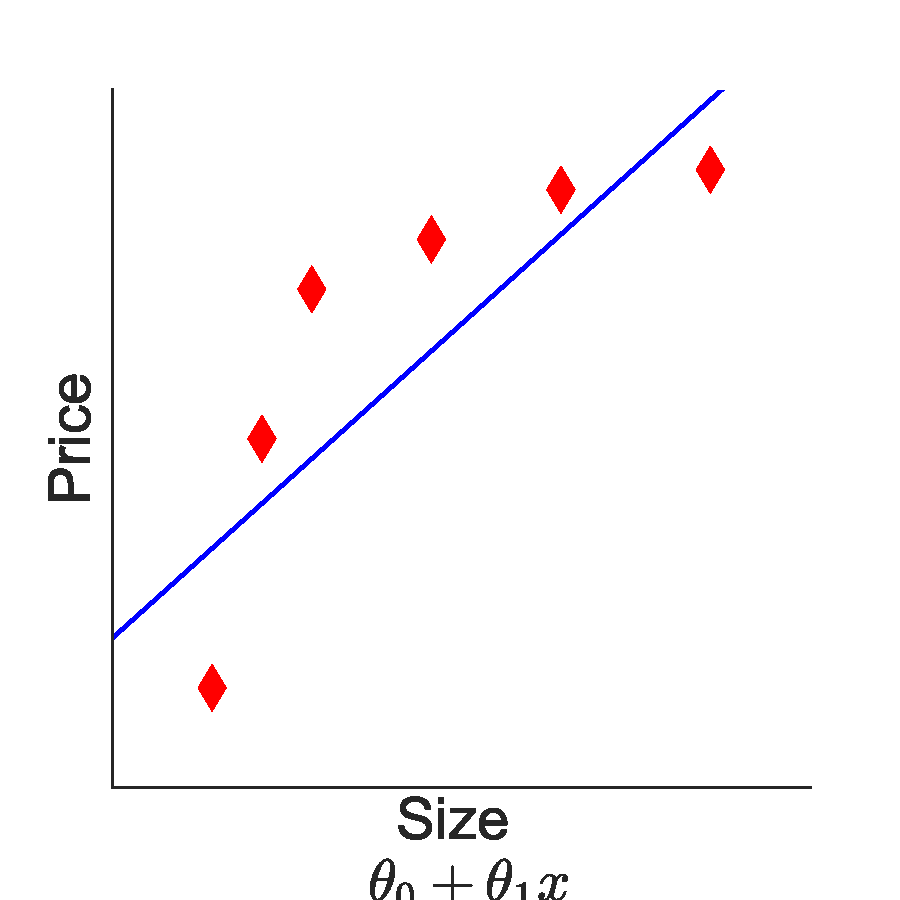
\includegraphics[scale=0.35]{logreg_eg7_housing_data_linreg.pdf} 
   		\caption[]{Linear Regression}
   		\label{logreg_eg7_housing_data_linreg.pdf}
	\end{subfigure}
	\begin{subfigure}[t]{0.3\textwidth}
   		\centering
    		\graphicspath{{./Figures/}}
   		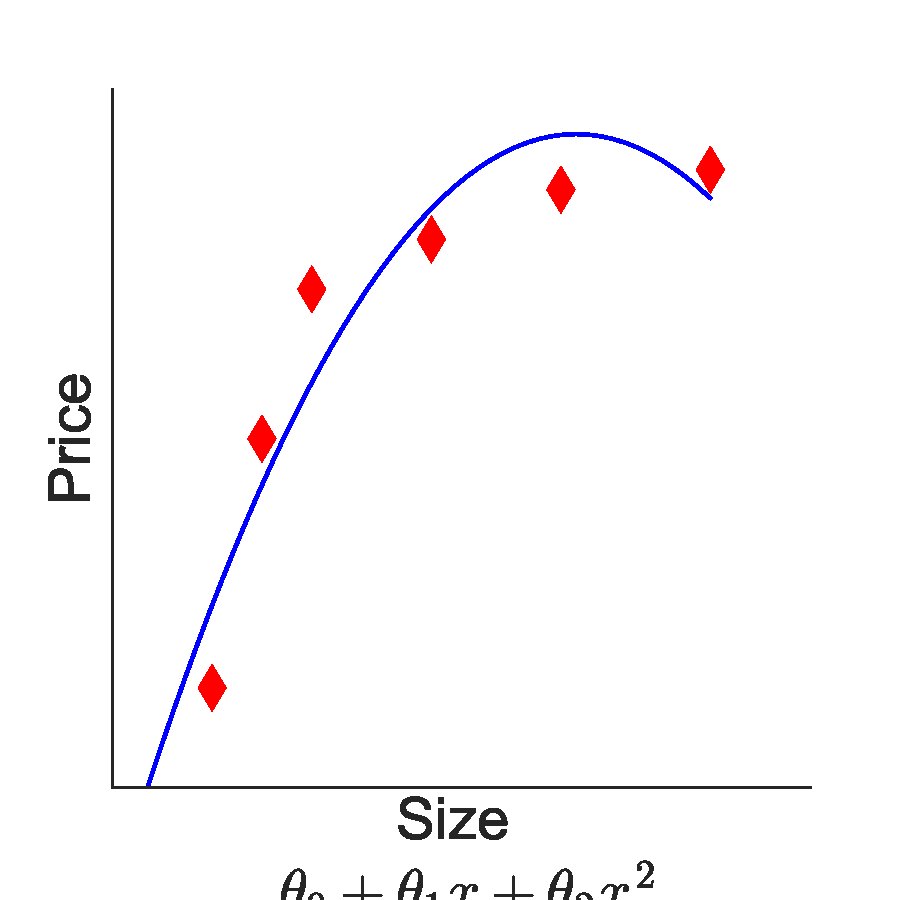
\includegraphics[scale=0.35]{logreg_eg7_housing_data_quadreg.pdf} 
   		\caption[]{Quadratic Regression}
   		\label{logreg_eg7_housing_data_quadreg.pdf}
	\end{subfigure}
	\begin{subfigure}[t]{0.3\textwidth}
   		\centering
    		\graphicspath{{./Figures/}}
   		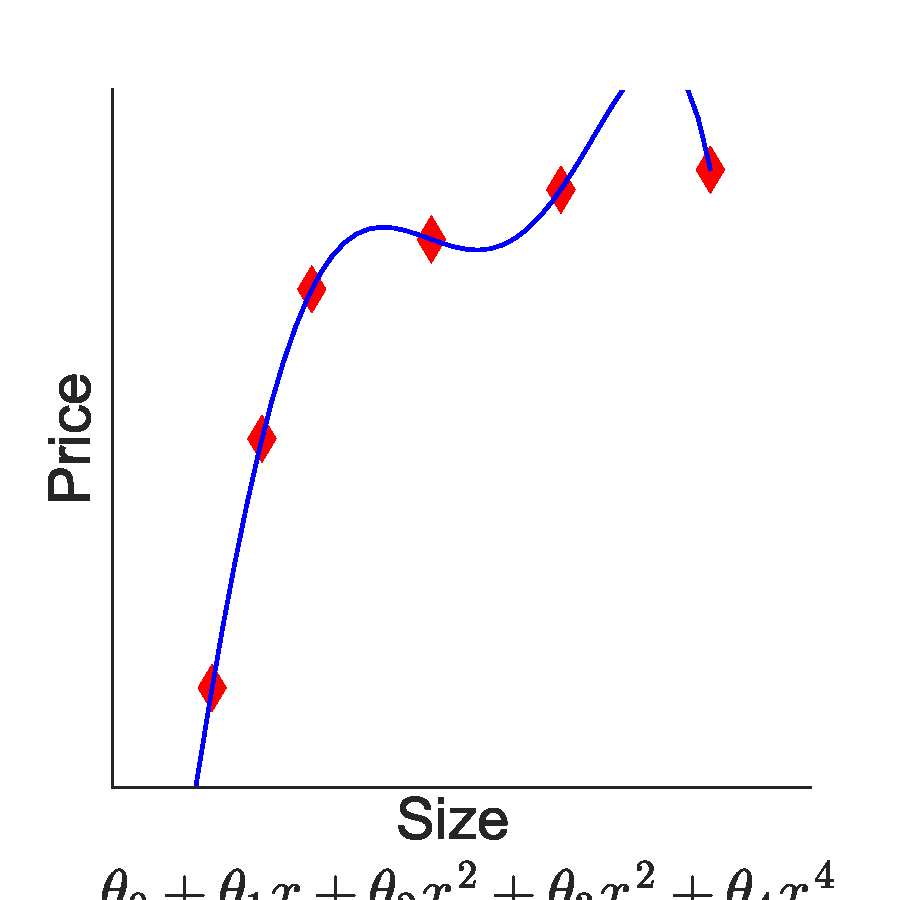
\includegraphics[scale=0.35]{logreg_eg7_housing_data_quadreg_overfit.pdf} 
   		\caption[]{Quadratic Regression with Additional Terms}
   		\label{logreg_eg7_housing_data_quadreg_overfit.pdf}
	\end{subfigure}
	\caption[]{Plots of linear and quadratic regressions with varying amounts of terms (features). }
%	\label{}
\end{figure}

Figure \ref{logreg_eg7_housing_data_linreg.pdf} is a linear regression on this data. This is the simplest regression, but looking at the data, it seems pretty clear that this isn't really a good fit. As the size of the house increases, the housing prices seem to plateau after a certain point, whereas the linear regression line keeps increasing. This is known as \textbf{underfitting}, or \textbf{high bias}.\footnote{The term \textit{bias} is somewhat or a historical or technical term. It carries with it the idea that if fitting a straight line to the data, it's as if the algorithm has a preconception (or bias) that the housing prices should vary linearly with their size, despite evidence in the data that this is not the case. Irrespective of the evidence to the contrary, the algorithm fits the data to a straight line, and it ends up not being a very good fit.} Both of these roughly mean that the regression just isn't fitting to the training data very well. In Figure \ref{logreg_eg7_housing_data_quadreg.pdf}, we can fit a quadratic function to the data. This seems to work pretty well, and looks like a better fit than the linear regression. Figure \ref{logreg_eg7_housing_data_quadreg_overfit.pdf} shows what happens when we \textbf{overfit} the line. This is also known as \textbf{high variance}. The curve fits the training set very well, but it particular to the specific training set, so it doesn't work well for any other data set. 

Let's formally define these terms now:
\begin{description}
\item[Overfitting] If we have too many features, the learned hypothesis may fit the training set very well ($J\left(\theta\right) \approx 0$), but fails to generalize to new examples. This is also called high variance. 
\item[Underfitting] This occurs when the form of our hypothesis function maps poorly to the trend of the data. It is usually caused by a function that is too simple or uses too few features. This is also called high bias. 
\end{description}
This apply to both linear and logistic regression. 

So how do we prevent our models from overfitting to the data? For the simple examples where we have one or two features, we can plot the data and determine it that way; but when we start working with data sets that have hundreds of features, this no longer works. We have two main options to address overfitting:
\begin{enumerate}
\item Reduce the number of features
	\begin{itemize}
	\item Manually select which features to keep, or
	\item Use a model selection algorithm (which we'll see later)
	\end{itemize}
\item Regularization
	\begin{itemize}
	\item Keep all the features, but reduce the parameters $\theta_j$
	\end{itemize}
\end{enumerate}
Regularization works well when we have a lot of slightly-useful features. 

\subsection{Cost Function}
If we suspect overfitting in our hypothesis function, we can reduce the weight of some of the terms in our function by increasing their cost. Say we have a hypothesis of the form
$$
h_\theta\left(x\right) = \theta_0 + \theta_1x + \theta_2x^2 + \theta_3x^3 + \theta_4x^4
$$
To reduce the effect of $\theta_3x^3$ and $\theta_4x^4$ without actually getting rid of those features, we instead modify our cost function to something like this
$$
\min_\theta \frac{1}{2m} \sum_{i=1}^m \left(h_\theta \left(x ^{\left(i\right)}\right) - y^{\left(i\right)}\right)^2 + 1000\left(\theta_3\right)^2 + 1000 \left(\theta_4\right)^2
$$
where $1000$ is an arbitrary large number that we chose. This inflates the cost of both $\theta_3$ and $\theta_4$, so to reduce our cost function, we end up reducing the values of $\theta_3$ and $\theta_4$ to near zero. This will greatly reduce the values of $\theta_3x^3$ and $\theta_4x^4$ in our hypothesis function. This usually yields a simpler hypothesis that is less prone to overfitting. 

In a more general sense, having small values for \textit{all} parameters typically decreases the likelihood that we'll overfit our regression. 

To implement regularization, we modify the cost function by adding a regularization term at the end to shrink every parameter, where $\lambda$ is called the regularization parameter. 
\begin{equation}
J_\theta = \frac{1}{2m}\left[ \sum_{i=1}^m \left(h_\theta\left( x^{(i)}\right) - y^{(i)}\right)^2 + \lambda\sum_{j=1}^n \theta_j^2\right]
\end{equation}
By convention, these summations start at $1$, so we don't regularize $\theta_0$. In this equation, the regularization parameter $\lambda$ controls the trade-off between two different goals: fitting the training data well (the first term of the equation), and keeping the parameters small (the regularization term). 

Conceptually, it can be somewhat difficult to see why keeping the parameters small reduces overfitting, but if you program this yourself, you'll see this effect firsthand. What actually happens is that by using the above cost function with regularization, the resulting output of the hypothesis function is smoothed out to reduce overfitting. However, if $\lambda$ is chosen to be too large, it may smooth out the function too much and underfit. For example, if $\lambda \sim 10^{10}$ for our housing data problem, then $\theta_j \to 0$ for $j \neq 0$.This leaves us with a regression that looks like $h_\theta\left(x\right) = \theta_0$, meaning our hypothesis is just a horizontal line. 


\subsection{Regularized Linear Regression}
We've previously looked at two algorithms for linear regression: one based on gradient descent, and one based on the normal equation. Now, we'll take these two algorithms and generalize them to regularized linear regression. Here is our cost function
\begin{equation}
J_\theta = \frac{1}{2m}\left[ \sum_{i=1}^m \left(h_\theta\left( x^{(i)}\right) - y^{(i)}\right)^2 + \lambda\sum_{j=1}^n \theta_j^2\right]
\end{equation}
and our goal is to get
\begin{equation}
\min_\theta J\left(\theta\right)
\end{equation}

\subsubsection{Gradient Descent}
Our standard gradient descent algorithms looks something like this:

\textbf{Repeat \{}
$$
\theta_j := \theta_j - \alpha \frac{1}{m} \sum_{i=1}^m \left( h_\theta\left(x^{(i)}\right) - y^{(i)}\right) x_j^{(i)} ~~\mbox{\;\;\;\;\;\;\;\;\;\; for } j = 0, 1, 2, \dots, n
$$
\textbf{\}} \\

\noindent To make this easier, we're just going to write the update for $\theta_0$ separately.

\textbf{Repeat \{}
\begin{subequations}
\begin{align}
\theta_0 &:= \theta_0 - \alpha \frac{1}{m} \sum_{i=1}^m \left( h_\theta\left(x^{(i)}\right) - y^{(i)}\right) x_0^{(i)} \\
\theta_j &:= \theta_j - \alpha \frac{1}{m} \sum_{i=1}^m \left( h_\theta\left(x^{(i)}\right) - y^{(i)}\right) x_j^{(i)} ~~\mbox{\;\;\;\;\;\;\;\;\;\; for } j = 1, 2, \dots, n \label{chaplogreg-sectregular-subsect-linreg-graddesc-oldeqtn}
\end{align}
\end{subequations}
\textbf{\}} \\
Now, we want to modify these equations to include our new regularization parameter. The $\theta_0$ equation stays the same since we don't regularize $\theta_0$, but equation \ref{chaplogreg-sectregular-subsect-linreg-graddesc-oldeqtn} becomes
\begin{subequations}
\begin{align}
\theta_0 &:= \theta_0 - \alpha \frac{1}{m} \sum_{i=1}^m \left( h_\theta\left(x^{(i)}\right) - y^{(i)}\right) x_0^{(i)} \\
\theta_j &:= \theta_j - \alpha \left[\frac{1}{m} \sum_{i=1}^m \left( h_\theta\left(x^{(i)}\right) - y^{(i)}\right) x_j^{(i)} + \frac{\lambda}{m}\theta_j \right] ~~\mbox{\;\;\;\;\;\;\;\;\;\; for } j = 1, 2, \dots, n \label{chaplogreg-sectregular-subsect-linreg-graddesc-neweqtn}
\end{align}
\end{subequations}
If you do the calculus out, you can prove that the large term in brackets in equation \ref{chaplogreg-sectregular-subsect-linreg-graddesc-neweqtn} is the partial derivative of the new $J\left(\theta\right)$ with the regularization term. 
$$
\frac{\partial}{\partial \theta_j} J\left(\theta\right)
$$
With some manipulation, we can rewrite our update rule as
\begin{equation}
\theta_j := \theta_j\left(1 - \alpha\frac{\lambda}{m}\right) - \alpha\frac{1}{m}\sum_{i=1}^m \left(h_\theta\left(x^{(i)}\right) - y^{(i)}\right) x_j^{(i)}
\end{equation}
where in the first term in the equation, the value $1 - \alpha\frac{\lambda}{m}$ will always be less than one. Intuitively, the term that's always less than one will serve to reduce $\theta_j$ by a small amount, and the other term is actually exactly the same as our previous gradient descent algorithm before we introduced regularization. 

\subsubsection{The Normal Equation}
Gradient descent was just one of the two algorithms we've explored as a solution to linear regression; the second algorithm was based on the normal equation. With the normal equation, we crafted the design matrix $X$ where each row corresponds to a separate training example, and we have an $m$-dimensional vector $\vec{y}$ that contains our labels. 
$$
X = \left[\begin{array}{c}
\left(x^{(1)}\right)^\intercal \\ \left(x^{(2)}\right)^\intercal \\ \vdots \\ \left(x^{(m)}\right)^\intercal
\end{array}\right] ~~\mbox{ \;\;\;\;\;\;\;\;\;\; }~~ \vec{y} = \left[\begin{array}{c} y^{(1)} \\ y^{(2)} \\ \vdots \\ y^{(m)} \end{array}\right]
$$
where we calculated the vector $\vec{\theta}$ as 
$$
\vec{\theta} = \left( X^\intercal X\right)^{-1} X^\intercal \vec{y}
$$
This minimized the unregularized cost function $J\left(\theta\right)$. To add in regularization, we add another term inside the parentheses
\begin{equation}
\vec{\theta} = \left( X^\intercal X + \lambda L \right)^{-1} X^\intercal \vec{y}
\end{equation}
where the matrix $L$ is a diagonal matrix\footnote{In linear algebra, a diagonal matrix is a matrix (usually a square matrix) in which the off-diagonal elements are all zero. The main diagonal entries themselves may or may not be zero.} given by:
\begin{equation}
L = \left[\begin{array}{cccccc}
0 &  &  &  &  &  \\
 & 1 & & & & \\
& & 1 & & & \\
& & & 1 & & \\
& & & & \ddots & \\
& & & & & 1
\end{array}\right]
\end{equation}
The matrix $L$ has $0$ in it's top left spot, then $1$'s down the diagonal and zeros everywhere else. It has dimensions $\left(n+1\right) \times \left(n+1\right)$. Intuitively, this is the identity matrix (sans $x_0$), multiplied by a single number $\lambda \in \mathbb{R}$.

Recall that if the number of examples $m \leq$ the number of features $n$, then $X^\intercal X$ is non-invertible.\footnote{A non-invertible square matrix is also called singular or degenerate.} We got around this programatically by using the pseudoinverse. Fortunately, regularization also takes care of this for us as well. As long as $\lambda \in \mathbb{R}_{>0}$ is strictly greater than zero, then $X^\intercal X + \lambda L$ will be strictly invertible. 


\subsection{Regularized Logistic Regression}
Logistic regression, just like linear regression, is prone to overfitting if you overfit with higher order polynomials. As we saw in equation \ref{chaplogreg-sectsimpcostfunct-simpcostfuncformula}, our logistic regression cost function is given by
$$
J\left(\theta\right) = -\frac{1}{m} \left[ \sum_{i=1}^m y^{\left(i\right)} \log h_\theta\left(x^{\left(i\right)}\right) + \left(1 - y^{\left(i\right)}\right) \log \left(1 - h_\theta\left(x^{\left(i\right)}\right)\right)\right]
$$
To morph this into a regularized equation, we need to add a regularization term at the end, resulting in
\begin{equation}
J\left(\theta\right) = -\frac{1}{m} \left[ \sum_{i=1}^m y^{\left(i\right)} \log h_\theta\left(x^{\left(i\right)}\right) + \left(1 - y^{\left(i\right)}\right) \log \left(1 - h_\theta\left(x^{\left(i\right)}\right)\right)\right] + \frac{\lambda}{2m}\sum_{j=1}^n \theta_j^2
\end{equation}
Note that in the second summation, $j \in \left[1, n\right]$, so this excludes $\theta_0$. 

In a similar fashion to what we did with linear regression, we're going to make the same changes to gradient descent for logistic regression. We start with our standard gradient descent equation (equation \ref{chaplogreg-sectcostfunct-subsectgraddscnt-logreggraddscnt}), and separate out the $\theta_0$ term into its own equation. This gives us the same initial result as linear regression. 
\begin{align}
\theta_0 &:= \theta_0 - \alpha \frac{1}{m} \sum_{i=1}^m \left( h_\theta\left(x^{(i)}\right) - y^{(i)}\right) x_0^{(i)} \\
\theta_j &:= \theta_j - \alpha \frac{1}{m} \sum_{i=1}^m \left( h_\theta\left(x^{(i)}\right) - y^{(i)}\right) x_j^{(i)} ~~\mbox{\;\;\;\;\;\;\;\;\;\; for } j = 1, 2, \dots, n 
\end{align}
Then, we again modify the second update rule
\begin{subequations}
\begin{align}
\theta_0 &:= \theta_0 - \alpha \frac{1}{m} \sum_{i=1}^m \left( h_\theta\left(x^{(i)}\right) - y^{(i)}\right) x_0^{(i)} \\
\theta_j &:= \theta_j - \alpha \left[\frac{1}{m} \sum_{i=1}^m \left( h_\theta\left(x^{(i)}\right) - y^{(i)}\right) x_j^{(i)} + \frac{\lambda}{m}\theta_j \right] ~~\mbox{\;\;\;\;\;\;\;\;\;\; for } j = 1, 2, \dots, n
\end{align}
\end{subequations}
Cosmetically, this is the same formula as for linear regression, but the hypothesis is different, so the equations end up being different. Again, the bracketed term is the new partial derivative of $J\left(\theta\right)$ with the regularized cost function. 














\section{Python Labs: Coding Logistic Regression in Python}
\section{Homework}





























\include{./Chapters/4-Regularization}


\appendix
\chapter{Notation}
\label{appendix:notation}

$
\begin{array}{cl}
\hat{{}} & \text{predicted output} \\
\hat{y} & \text{predicted output of the variable $y$} \\


%%%%%%%%%%%
\\ \\ \\ \\ 
\mathbb{Z} & \text{the set of integers; zahlen is the German word for numbers} \\
\bigoplus & \mathrm{the\;earth} \\
\bigodot & \mathrm{the\;sun} \\
c & \mathrm{speed\;of\;light}\\
G & \mathrm{Newton's\;gravitational\;constant} \\
C & \mathrm{circumference} \\
S & \mathrm{distance} \\
\end{array}
$
\chapter{Linear Algebra Review}

\end{document}
